\documentclass[11pt]{report}
\usepackage[utf8]{inputenc}
\usepackage{amsmath, amssymb}
\usepackage{listings}
\usepackage{xcolor}
\usepackage{a4wide}
\usepackage{epsfig}
\usepackage{amssymb}
\usepackage{amsmath}
\usepackage{minted}
\usepackage{enumerate}
\usepackage{fancyvrb}
\usepackage{alltt}
\usepackage{fleqn}
\usepackage{epic}
\usepackage{color} 
\usepackage{theorem}
\usepackage{hyperref}
\usepackage{tikz}

\usepackage{newunicodechar}

\newunicodechar{→}{\ensuremath{\rightarrow}}
\newunicodechar{←}{\ensuremath{\leftarrow}}
\newunicodechar{⇒}{\ensuremath{\Rightarrow}}

\newunicodechar{∈}{\ensuremath{\in}}
\newunicodechar{∉}{\ensuremath{\notin}}
\newunicodechar{∪}{\ensuremath{\cup}}
\newunicodechar{∩}{\ensuremath{\cap}}

\usepackage[all]{hypcap}
\hypersetup{
        colorlinks = true, % comment this to make xdvi work
        linkcolor  = blue,
        citecolor  = red,
        filecolor  = [rgb]{0.1, 0.1, 1.0},
        urlcolor   = [rgb]{0.7, 0.0, 0.7},
        pdfborder  = {0 0 0} 
}

\usepackage{fancyhdr}
\usepackage{lastpage} 

\definecolor{bg}{rgb}{0.9,0.8,0.6}
\definecolor{amber}{rgb}{1.0, 0.75, 0.0}
\definecolor{gold}{rgb}{1.0, 0.843, 0.0}

% Set up listings for Python
\lstset{
    language=Python,
    basicstyle=\ttfamily\small,
    keywordstyle=\color{blue},
    stringstyle=\color{red},
    commentstyle=\color{green!60!black},
    showstringspaces=false,
    breaklines=true,
    frame=single,
    captionpos=b
}

\pagestyle{fancy}

\fancyfoot[C]{--- \thepage/\pageref{LastPage}\ ---}

\fancypagestyle{plain}{%
\fancyhf{}
\fancyfoot[C]{--- \thepage/\pageref{LastPage}\ ---}
\renewcommand{\headrulewidth}{0pt}
}

\renewcommand{\chaptermark}[1]{\markboth{\chaptername \ \thechapter.\ #1}{}}
\renewcommand{\sectionmark}[1]{\markright{\thesection. \ #1}{}}
\fancyhead[R]{\leftmark}
\fancyhead[L]{\rightmark}

\definecolor{amethyst}{rgb}{0.2, 0.4, 0.6}
\definecolor{orange}{rgb}{1, 0.9, 0.0}

\definecolor{codegray}{rgb}{0.5,0.5,0.5}
\definecolor{codepurple}{rgb}{0.58,0,0.82}
\definecolor{backcolour}{rgb}{0.95,0.95,0.92}

\lstdefinestyle{haskellstyle}{
    backgroundcolor=\color{backcolour},   
    commentstyle=\color{codegray},
    keywordstyle=\color{blue},
    numberstyle=\tiny\color{codegray},
    stringstyle=\color{codepurple},
    basicstyle=\ttfamily\footnotesize,
    breakatwhitespace=false,         
    breaklines=true,                 
    captionpos=b,                    
    keepspaces=true,                 
    numbers=left,                    
    numbersep=5pt,                  
    showspaces=false,                
    showstringspaces=false,
    showtabs=false,                  
    tabsize=2
}

{\theorembodyfont{\sf}
\newtheorem{Definition}{Definition}
\newtheorem{Axiom}[Definition]{Axiom}
\newtheorem{Notation}[Definition]{Notation}
\newtheorem{Theorem}[Definition]{Theorem}
}

\newcommand{\squote}[1]{\texttt{\symbol{34}#1\symbol{34}}}
\newcommand{\blue}[1]{{\color{blue}#1}}


\newcommand{\qed}{\hspace*{\fill} $\Box$
\vspace*{0.2cm}

}

\newcommand{\eod}{\hspace*{\fill} $\diamond$}
\newcommand{\eox}{\hspace*{\fill} $\diamond$}

\newcommand{\dangersign}[1][Danger]{
    \begin{tikzpicture}[scale=0.7]
        % Draw the triangle
        \draw[thick, red, fill=yellow] (0,0) -- (2,3.46) -- (4,0) -- cycle;
        % Add the text (default is "Danger")
        \node at (2,0.8) {\textbf{\textsc{#1}}};
    \end{tikzpicture}
}

\newcommand{\wip}[1][\ \ Work in Progress!]{
    \begin{tikzpicture}[scale=0.7]
        % Draw rectancle
        \draw[thick, blue, fill=orange] (0,3) -- (6.5, 3) -- (6.5,4) -- (0, 4) -- cycle;
        \node at (3,3.5) {\textbf{\textsc{#1}}};
    \end{tikzpicture}
}
\title{
\epsfig{file=dhbw-logo.pdf, scale=1.5}\\[0.3cm]  
       Functional Programming in \textsl{Haskell} \\[0.3cm]
      --- Winter 2025 ---}
\author{Prof.~Dr.~Karl Stroetmann}
\date{\today \\[1.5cm]
  \dangersign \wip \dangersign
}

\newcommand{\ds}{\displaystyle}
\newcommand{\solution}{\vspace*{0.2cm}

\noindent
\textbf{Solution}: }

\newcounter{aufgabe}
\newcommand{\exercise}{\vspace*{0.2cm}
\stepcounter{aufgabe}

\noindent
\textbf{Exercise \arabic{aufgabe}}: }

\newcommand{\exerciseStar}{\vspace*{0.2cm}
\stepcounter{aufgabe}

\noindent
\textbf{Exercise \arabic{aufgabe}$^*$}: }


\newcommand{\example}{\vspace*{0.2cm}

\noindent
\textbf{Example}: \ }

\newcommand{\examples}{\vspace*{0.2cm}

\noindent
\textbf{Examples}: \ }
 
\newcommand{\remark}{\vspace*{0.2cm}
\noindent
\textbf{Remark}: }

\newcommand{\lb}{\hspace*{\fill} \linebreak}


\def\pair(#1,#2){\langle #1, #2 \rangle}

\newlength{\mylength}
\setlength{\mathindent}{1.3cm}

\begin{document}
\maketitle
\tableofcontents

\begin{abstract}
\noindent
This is a very short introduction to functional programming with
\href{https://en.wikipedia.org/wiki/Haskell}{\textsl{Haskell}}. 
It is not intended to be a Haskell course.  My intention merely is for the reader to get a taste of what
programming in \textsl{Haskell} feels like.  If I succeed in convincing the reader that \textsl{Haskell} is a
programming language that is both usefull and mind extending, then I consider my job done.
Therefore, this short paper will just present some of the highlights of the programming language
\textsl{Haskell} via examples that I hope the reader finds intriguing enough so that she feels inclined to read
some of the outstanding books introducing Haskell in more depth.  There are three books that I recommend for
those readers who want to understand \textsl{Haskell} in more depth:  
\begin{enumerate}
\item \emph{Programming in Haskell}

      by Graham Hutton \cite{hutton:2016}.  This book has some nice \href{https://www.youtube.com/playlist?list=PLF1Z-APd9zK7usPMx3LGMZEHrECUGodd3}{YouTube videos}.
\item \emph{Haskell: The Craft of Functional Programming}

      by Simon Thompson \cite{thompson:2011}.
      This book is available free online at
      \\[0.2cm]
      \hspace*{1.3cm}
      \href{https://www.haskellcraft.com}{https://www.haskellcraft.com}.

\item \emph{Learn You a Haskell for Great Good!}

      by Miran Lipova\v{c}a \cite{lipovaca:2011}.
      This book is available free online at
      \\[0.2cm]
      \hspace*{1.3cm}
      \href{https://learnyouahaskell.com/}{https://learnyouahaskell.com}.
\item \emph{Effective Haskell: Solving Real-World Problems with Strongly Typed Functional Programming} 

      by Rebecca Skinner \cite{skinner:2023}.
\end{enumerate}
\end{abstract}

\chapter{Introduction}
In this introduction I will do two things:
\begin{enumerate}
\item First, I discuss those features of Haskell that set Haskell apart from other programming languages.
\item Second, I will present a few short example programs that give a first taste of Haskell.
\end{enumerate}

\section{Why Haskell is Different}
Before we present any details of \textsl{Haskell}, let us categorize this programming language so that we have
an idea about what to expect.  \textsl{Haskell} has the following properties:
\begin{enumerate}
\item \textsl{Haskell} is a \blue{functional programming language}.

  A functional programming language is any programming language that treats functions as
  \blue{first class citiziens}:
  \begin{enumerate}
  \item A function can be given as an argument to another function.
  \item A function can be produce a function as its result.
  \end{enumerate}
  A well known programming language that supports functional programming is \textsl{Python} and there are
  several books discussing functional programming in \textsl{Python}, e.g.~\cite{lott:2022}, \cite{mertz:2015},
  and \cite{reid:2023}.  

\item \textsl{Haskell} is \blue{statically typed}.

  Every variable in Haskell has a fixed type, which can not be changed.  In this respect, \textsl{Haskell} is
  similar to the programming language \textsl{Java}.  However, in contrast to \textsl{Java}, we do not have to
  declare the type of every variable and every function because most of the time the type of a variable can be
  \blue{inferred} by the type system.  Therefore, in Haskell we usually specify only the types of non-trivial
  functions.

  The benefit of this approach is that many type errors will already be caught by the compiler.  This is in
  contrast to programs written in a dynamically typed language like \textsl{Python}, where type errors are only
  discovered at runtime.

\item \textsl{Haskell} is a \blue{pure} functional programming language.

  Once a variable is assigned a value, this value can not be changed.  For example, if we want to sort a list,
  we are not able to change the list data structure.  All we can do is to compute a new list which contains the
  same elements as the old list and which, furthermore, is sorted.

  The property of being a \blue{pure} language sets \textsl{Haskell} apart from most other programming
  languages.  Even the language
  \href{https://en.wikipedia.org/wiki/Scala_(programming_language)}{\textsl{Scala}}, which is designed as a
  modern functional programming language, is not pure.

  What is the big deal about purity?  On one hand, it forces
  the user to program in a declarative style.  Although, in general, nobody likes to be forced to do something,
  there is a huge benefit in pure programming.
  \begin{enumerate}
  \item In a pure programming language, functions will always return the same result when they are called with
    the same arguments.  This property is called \blue{referential transparency}.
    This makes reasoning about code easier, as you can replace a function call with its result without changing
    the behavior of the program.  Therefore the correctness of functions can be verified mathematically.
  \item Since pure functions do not depend on or modify external state, their behavior is entirely predictable.
    The advantage is that testing becomes straightforward because functions can be tested in isolation without
    worrying about interactions with other parts of the system. 
  \item Compilers for pure languages can make aggressive optimizations, such as caching function results
    (\blue{memoization}) or reordering computations, because they know that functions are side-effect-free. 
    The advantage is that programs can often run faster.
  \item Furthermore, \blue{concurrency} becomes much easier to manage when functions do not use global variables and do
    not change their arguments.
  \end{enumerate}
  
\item \textsl{Haskell} is a \blue{compiled} language similar to \textsl{Java} and \texttt{C}, but additionally
  offers an interpreter.  Having an interpreter is beneficial for rapid prototyping.  The property that
  \textsl{Haskell} programs can be compiled ensures that the resulting programs can befaster than,
  for example, \textsl{Python} programs.
\item \textsl{Haskell} is a \blue{lazy} language.  The programming language \texttt{C} is an \blue{eager}
  language.  If an expression  of the form
  \\[0.2cm]
  \hspace*{1.3cm}
  $f(a_1, \cdots, a_n)$
  \\[0.2cm]
  has to be evaluated, first the subexpressions $a_1$, $\cdots$ $a_n$ are evaluated.  Let us assume that $a_i$
  is evaluated to to value $x_i$.  The, $f(x_1, \cdots, x_n)$ is computed.  This might be very inefficient.
  Consider the example shown in Figure \ref{fig:eager.c} on page \pageref{fig:eager.c}.

\begin{figure}[!ht]
  \centering
\begin{minted}[ frame         = lines, 
                 framesep      = 0.3cm, 
                 firstnumber   = 1,
                 bgcolor       = bg,
                 numbers       = left,
                 numbersep     = -0.2cm,
                 xleftmargin   = 0.8cm,
                 xrightmargin  = 0.8cm,
               ]{C}
  int f(int x, int y) {
      if (x == 2) {
          return 42;
      }
      return 2 * y;
  }
\end{minted}
\vspace*{-0.3cm}
\caption{A \texttt{C} program.}
\label{fig:eager.c}
\end{figure}

Let us assume that the expression
\\[0.2cm]
\hspace*{1.3cm}
\texttt{f(h(0), g(1))}
\\[0.2cm]
needs to be evaluated and that the computation of \texttt{g(1)} is very expensive.  In a
\texttt{C}-program, the expressions and \texttt{h(0)} and \texttt{g(1)} will be both evaluated.  If it turns out that
\texttt{h(0)} is \texttt{2}, then the evaluation of \texttt{g(1)} is not really necessary.  Nevertheless, in \texttt{C} this
evaluation takes place because \texttt{C} has an \blue{eager} evaluation strategy.  In contrast, an equivalent
\textsl{Haskell} would not evaluate the expression \texttt{h(0)} and hence would be much more efficient.

\item \textsl{Haskell} is difficult to learn.

  You might ask yourself why \textsl{Haskell} hasn't been adopted more widely.  After all, it has all these
  cool features mentioned above.  The reason is that learning \textsl{Haskell} is a lot more difficult then
  learning a language like \textsl{Python} or \textsl{Java}.  There are two reasons for this:
  \begin{enumerate}[(a)]
  \item First, \textsl{Haskell} differs a lot from those languages that most people know.
  \item In order to be very concise, the syntax of \textsl{Haskell} is quite different from the syntax of
        established programming languages.
  \item \textsl{Haskell} requires the programmer to think on a very high level of abstraction.
        Many students find this difficult.
  \item Lastly, and most importantly, \textsl{Haskell} supports the use of a number of concepts
        like, e.g.~\href{https://en.wikipedia.org/wiki/Functor}{functors} and
        \href{https://en.wikipedia.org/wiki/Monad_(category_theory)}{monads} from 
        \href{https://en.wikipedia.org/wiki/Category_theory}{category theory}. 
        It takes both time and mathematical maturity to really understand these concepts.

        If you really want to understand the depth of \textsl{Haskell}, you have to dive into those topics.
        That said, while you have to understands both functors and monads, you do not have to understand
        category theory.
  \item Fortunately, it is possible to become productive in \textsl{Haskell} without understanding 
        functors and monads.  Therefore, this lecture will focuss on those parts of \textsl{Haskell} that are more easily
        accessible. 
  \end{enumerate}
\end{enumerate}

\section{A First Taste of Haskell}
\subsubsection{Computing All Prime Numbers}
A \href{https://en.wikipedia.org/wiki/Prime_number}{prime number} is a natural number $p$ that is different from $1$
and that can not be written as a product of two natural numbers $a$ and $b$ that are both different from $1$.  If
we denote the set of all prime numbers with the symbol $\mathbb{P}$, we therefore have:
\\[0.2cm]
\hspace*{1.3cm}
$\ds \mathbb{P} = \bigl\{ p \in \mathbb{N} \mid n \not= 1 \wedge \forall a, b \in \mathbb{N}:(a \cdot b = p
\implies a = 1 \vee b = 1) \bigr\}$
\\[0.2cm]
An efficient method to compute the prime numbers is the
\href{https://en.wikipedia.org/wiki/Sieve_of_Eratosthenes}{sieve of Eratosthenes}.
This is an algorithm used to find all primes up to a given number. The method works by iteratively marking the
multiples of each prime number starting from 2. The numbers which remain unmarked at the end of the process are
the prime numbers.  For example, consider the list of integers from 2 to 30:
\\[0.2cm]
\hspace*{0.3cm}
$2, 3, 4, 5, 6, 7, 8, 9, 10, 11, 12, 13, 14, 15, 16, 17, 18, 19, 20, 21, 22, 23, 24, 25, 26, 27, 28, 29, 30$.
\\[0.2cm]
We will now compute the set of all primes less or equal than 30 using the Sieve of Eratosthenes.
\begin{enumerate}
\item The first number in this list is $2$ and hence $2$ is prime:
      \\[0.2cm]
      \hspace*{1.3cm}
      $\mathbb{P} = \{ 2, \cdots \}$.
\item We remove all multiples of 2 (i.e., 2, 4, 6, 8, \(\ldots\), 30).  This leaves us with the list
      \\[0.2cm]
      \hspace*{1.3cm}
      $3, 5, 7, 9, 11, 13, 15, 17, 19, 21, 23, 25, 27, 29$.
      \\[0.2cm]
      The first remaining number $3$ is prime.  Hence we have
      \\[0.2cm]
      \hspace*{1.3cm}
      $\mathbb{P} = \{ 2, 3, \cdots \}$
\item We remove all multiples of 3 (i.e., 3, 6, 9, 12, \(\ldots\), 27).  Note that some numbers (like 6 or 12,
      for instance) may already have been removed.  This leaves us with the list
      \\[0.2cm]
      \hspace*{1.3cm}
      $5, 7, 11, 13, 17, 19, 23, 25, 29$.
      \\[0.2cm]
      The first remaining number $5$ is prime. Hence we have
      \\[0.2cm]
      \hspace*{1.3cm}
      $\mathbb{P} = \{ 2, 3, 5, \cdots \}$.
\item We remove all multiples of 5 (i.e., 5, 10, 15, 20, \(\ldots\)). This leaves us with the list
      \\[0.2cm]
      \hspace*{1.3cm}
      $7, 11, 13, 17, 19, 23, 29$.
      \\[0.2cm]
      The first remaining number $7$ is prime. Hence we have
      \\[0.2cm]
      \hspace*{1.3cm}
      $\mathbb{P} = \{ 2, 3, 5, 7, \cdots \}$.
\item Since the square of $7$ is $49$, which is greater that 30, there is no need to remove the multiples of
      $7$,  since all multiples $a \cdot 7$ for $a < 7$ have already been removed and all multiples $a \cdot 7$
      for $a \geq 7$ are greater than 30. Hence the remaining numbers are all prime and we have found that the
      prime numbers less or equal than 30 are: 
      \\[0.2cm]
      \hspace*{1.3cm}
      $\{ 2, 3, 5, 7, 11, 13, 17, 19, 23, 29\}$. 
\end{enumerate}

\begin{figure}[!ht]
\centering
\begin{minted}[ frame         = lines, 
                 framesep      = 0.3cm, 
                 firstnumber   = 1,
                 bgcolor       = bg,
                 numbers       = left,
                 numbersep     = -0.2cm,
                 xleftmargin   = 0.8cm,
                 xrightmargin  = 0.8cm,
               ]{python3}
def sieve_of_eratosthenes(n):
    """Return a list of prime numbers up to n (inclusive)."""
    if n < 2:
        return []    
    is_prime = [True] * (n + 1)
    is_prime[0] = is_prime[1] = False  # 0 and 1 are not primes
    p = 2
    while p * p <= n:
        if is_prime[p]:
            for i in range(p * p, n + 1, p):
                is_prime[i] = False
        p += 1
    return [i for i, prime in enumerate(is_prime) if prime]
\end{minted}
\vspace*{-0.3cm}
\caption{A \textsl{Python program to compute the prime numbers up to $n$.}}
\label{fig:primes.py}
\end{figure}
Figure \ref{fig:primes.py} on page \pageref{fig:primes.py} shows a Python script that implements the Sieve of
Eratosthenes to compute all prime numbers up to a limit \texttt{n}.  This script first initializes the list
\texttt{is\_prime} to track prime status. It then iteratively marks the multiples of each prime number, finally
collecting and printing all numbers that remain marked as prime.  This script implements one optimization: If
\texttt{p} is a prime, then only the multiples of \texttt{p} that have the form $a \cdot \mathtt{p}$ with
$a \geq \mathtt{p}$ have to be removed from the list, since a product of the form $a \cdot \mathtt{p}$ with
$a < \mathtt{p}$ has already been removed when removing multiples  
of $a$ or, if $a$ is not prime, of multiples of whatever prime is contained in $a$.



\begin{figure}[!ht]
\centering
\begin{minted}[ frame         = lines, 
                 framesep      = 0.3cm, 
                 firstnumber   = 1,
                 bgcolor       = bg,
                 numbers       = left,
                 numbersep     = -0.2cm,
                 xleftmargin   = 0.8cm,
                 xrightmargin  = 0.8cm,
               ]{haskell}
    primes :: [Integer]
    primes = sieve [2..]
    
    sieve :: [Integer] -> [Integer]
    sieve (p:ns) = p : sieve [n | n <- ns, mod n p /= 0]
\end{minted}
\vspace*{-0.3cm}
\caption{Computing the prime numbers.}
\label{fig:primes.hs}
\end{figure}

Figure \ref{fig:primes.hs} on page \pageref{fig:primes.hs} shows a \textsl{Haskell} program to compute \textbf{all}
primes.  Yes, you have read that correct.  It doesn't compute the primes up to a given number, but rather it
computes \underline{all} primes.

The first thing to note is that line 1 and line 4 are type annotations.  They have only
been added to aid us in understanding the program.  If we would drop these lines, the program would still
work.  Hence, we have an efficient 2-line program to compute the prime numers.  Lets discuss this program line
by line. 
\begin{enumerate}[(a)]
\item Line 1 states that the function \texttt{primes} returns a list of \texttt{Integer}s.
  \texttt{Integer} is the type of all arbitrary precision integers.  The fact that we have enclosed
  the type name \texttt{Integer} in the square brackets ``\texttt{[}'' and ``\texttt{]}'' denotes that the
  result has the type \textsl{list} of \texttt{Integer}.
\item In line 2, the expression ``\texttt{[2..]}''  denotes the list of all integers starting from $2$.  Since
  \textsl{Haskell} is lazy, it is able to support infinite data structures.  The trick is that these lists are
  only evaluated as much as they are needed.  As long as we do not inspect the complete list, everything works
  fine. 
\item Line 2 calls the function \texttt{sieve} with the argument \texttt{[2..]}.  \textsl{Haskell} uses prefix
  notation for calling a function.  If $f$ is a function an $a_1$, $a_2$, and $a_3$ are arguments of this
  function, then the invocation of $f$ with these arguments is written as
  \\[0.2cm]
  \hspace*{1.3cm}
  $f$ $a_1$ $a_2$ $a_3$
  \\[0.2cm]
  \textbf{Note} that the expression
  \\[0.2cm]
  \hspace*{1.3cm}
  $f(a_1, a_2, a_3)$
  \\[0.2cm]
  denotes something different:  This expression would apply the function $f$ to a single argument, which is the
  triple $(a_1, a_2, a_3)$.
\item Line 4 declares the type of the function \texttt{sieve}.  This function takes one argument, which is a
  list of \texttt{Integer}s and returns a list of \texttt{Integer}s.
\item Line 5 defines the function \texttt{sieve} that takes a list of numbers $l$ that has the following
  properties:
  \begin{itemize}
  \item The list $l$ is a sorted ascendingly.
  \item If $p$ is the first element of the list $l$, then $p$ is a prime number.
  \item The list $l$ does not contain multiples of any number $q$ that is less than $p$:
    \\[0.2cm]
    \hspace*{1.3cm}
    $\forall q \in \mathbb{N}: \bigl(q < p \rightarrow \forall n \in \mathbb{N}: n \cdot q \not\in l\bigr)$.
  \end{itemize}
  Given a list $l$ with these properties, the expression
  \\[0.2cm]
  \hspace*{1.3cm}
  \texttt{sieve l}
  \\[0.2cm]
  returns a list of all prime number that are greater or equal than $p$, where $p$ is the first element of $l$: 
  \\[0.2cm]
  \hspace*{1.3cm}
  $\mathtt{sieve}\;l = [\; q \in l \mid q \in \mathbb{P}\;]$.
  \\[0.2cm]
  Hence, when \texttt{sieve} is called with the list of all natural number greater or equal than $2$
  it will return the list of all prime numbers, since $2$ is the smallest  prime numer.

  There is a lot going on in the definition of the function \texttt{sieve}.  We will discuss this definition
  in minute detail.
  \begin{enumerate}[1.]
  \item The function \texttt{sieve} is defined via \blue{matching}.  We will discuss matching in more detail in
    the next chapter.  For now we just mention that the expression
    \\[0.2cm]
    \hspace*{1.3cm}
    \texttt{(p:ns)}
    \\[0.2cm]
    matches a list with first element \texttt{p}.  The remaining elements are collected in the list
    \texttt{ns}.  For example, if \texttt{l = [2..]}, i.e.~if $l$ is the list of all natural numbers greater or
    equal than $2$, then the variable \texttt{p} is bound to the number $2$, while the variable \texttt{ns} is
    bound to the list of all natural numbers greater or equal than $3$, i.e.~\texttt{ns = [3..]}.
  \item The right hand side of the function definition, i.e.~the part after the symbol ``\texttt{=}'' defines the
    value that is computed by the function \texttt{sieve}.  This value is computed by calling the function
    ``\texttt{:}'', which is also known as the \blue{cons} function because it \underline{cons}tructs a list.
    The operator ``\texttt{:}'' takes two arguments.  The first argument is a value \texttt{u} of some type $a$
    and the second argument \texttt{us} is list of elements of the same type $a$.  An expression of the form
    \\[0.2cm]
    \hspace*{1.3cm}
    \texttt{u :\;us}
    \\[0.2cm]
    then returns a list where \texttt{u} is the first elements and \texttt{us} are the remaining elements.
    For example, we have
    \\[0.2cm]
    \hspace*{1.3cm}
    \texttt{1 :\;[2, 3, 4] = [1, 2, 3, 4]}.
  \item The recursive invocation of the function sieve takes a \blue{list comprehension} as ist first argument.
    the expression
    \\[0.2cm]
    \hspace*{1.3cm}
    \texttt{[n | n <- ns, mod n p /= 0]}
    \\[0.2cm]
    computes the list of all those number \texttt{n} from the list \texttt{ns} that have a non-zero remainder
    when divided by the prime number \texttt{p}, i.e.~this list contains all those number from the list
    \texttt{ns} that are not multiples of \texttt{p}.  There are two things to note here concerning the syntax
    of \textsl{Haskell}:
    \begin{itemize}
    \item Functions are written with prefix notation.  For example, we first write the function name
      \texttt{mode} followed by the arguments \texttt{m} and \texttt{p}.  In \textsl{Python} the expression
      \\[0.2cm]
      \hspace*{1.3cm}
      \texttt{mod m p}
      \\[0.2cm]
      would have been written as \ \texttt{m \% p}.
    \item The operator ``\texttt{/=}'' expresses inequality, i.e.~the \textsl{Haskell} expression
      \\[0.2cm]
      \hspace*{1.3cm}
      \texttt{a /= b} \qquad would be written as \qquad \texttt{a != b} 
      \\[0.2cm]
      in the programming language \textsl{Python}.
    \end{itemize}
    Putting everything together, the \textsl{Haskell} expression 
    \\[0.2cm]
    \hspace*{1.3cm}
    \texttt{[n | n <- ns, mod n p /= 0]}
    \\[0.2cm]
    is therefore equivalent to the \textsl{Python} expression
    \\[0.2cm]
    \hspace*{1.3cm}
    \texttt{[n for n in ns if n \% p != 0]}.
  \end{enumerate}
\end{enumerate}

%%% Local Variables:
%%% mode: latex
%%% TeX-master: "haskell"
%%% End:

\chapter{Types, Expressions, and Functions}
In this Chapter we will give a more systematic overview of \textsl{Haskell}.  In particular, we define
\begin{enumerate}
\item types, 
\item expressions, and
\item functions.
\end{enumerate}
At this point you might wonder why we don't also discuss statements and control structures.  The reason is
simple:  There are no statements in \textsl{Haskell}. Everything is an expression.  Neither are there control
structures. 

\textsl{Haskell} is a statically typed, purely functional programming language known for its expressive type
system and emphasis on immutability. In \textsl{Haskell}, types play a central role in the design and
implementation of programs. This section discusses the primitive types available in \textsl{Haskell}, their
properties, and how they form the building blocks for more complex types in the language. 

Primitive types in \textsl{Haskell} refer to the basic types that are built into the language and directly
supported by the compiler. These types include numbers, characters, booleans, and the unit type. Understanding
these types is crucial for both writing correct programs and for taking full advantage of \textsl{Haskell}'s
type system. 

\section{Primitive Types}
\textsl{Haskell} provides several predefined types, each serving different needs with respect to performance, precision,
and range. The main numeric types in \textsl{Haskell} include: 
\begin{enumerate}[(a)]
\item \texttt{Int} is a fixed-precision integer type, which means that its range is limited by the underlying
      hardware. Typically, \texttt{Int} is implemented as a 32-bit or 64-bit integer. Its limited range means that
      operations on very lar~ge numbers may result in overflow. 

      \paragraph{Example Usage:}
      \begin{lstlisting}[style=haskellstyle, language=Haskell]
 -- Defining an integer of type Int
 smallInt :: Int
 smallInt = 42
      \end{lstlisting}

\item \texttt{Integer} represents arbitrary-precision integers. This means that there is no fixed upper bound
      on the size of an \texttt{Integer} value, though operations may become slower as numbers grow larger. 

\paragraph{Example Usage:}
\begin{lstlisting}[style=haskellstyle, language=Haskell]
-- Defining an integer of type Integer
bigInt :: Integer
bigInt = 123456789012345678901234567890
\end{lstlisting}

\item \texttt{Float} is the type of single-precision floating-point numbers. While it may be faster and uses less
      memory, its precision is limited compared to \texttt{Double}. 

\paragraph{Example Usage:}
\begin{lstlisting}[style=haskellstyle, language=Haskell]
-- Defining a floating-point number of type Float
singlePrecision :: Float
singlePrecision = 3.14159
\end{lstlisting}

\item \texttt{Double} is a double-precision floating-point number, offering more precision at the cost of
      additional memory and potentially slower computation in some contexts. 

\paragraph{Example Usage:}
\begin{lstlisting}[style=haskellstyle, language=Haskell]
-- Defining a floating-point number of type Double
doublePrecision :: Double
doublePrecision = 2.718281828459045
\end{lstlisting}

\item \texttt{Char} is used to represent single Unicode characters. Characters in \textsl{Haskell} are enclosed
      in single quotes. 

\paragraph{Example Usage:}
\begin{lstlisting}[style=haskellstyle, language=Haskell]
-- A character literal
letterA :: Char
letterA = 'A'
\end{lstlisting}

\item \texttt{String} is used to represent Unicode strings.  In \textsl{Haskell}, strings are enclosed in double quotes.

\paragraph{Example Usage:}
\begin{lstlisting}[style=haskellstyle, language=Haskell]
-- A string literal
letterA :: Char
letterA = "Hello, World!"
\end{lstlisting}
In \textsl{Haskell} the type \texttt{String} is an alias for the type \texttt{[Char]}, which represents a list
of characters.

\item \texttt{Bool} represents boolean values. It has two possible values: \texttt{True} and \texttt{False}.

\paragraph{Example Usage:}
\begin{lstlisting}[style=haskellstyle, language=Haskell]
-- A boolean literal
isHaskellFun :: Bool
isHaskellFun = True
\end{lstlisting}

\item The \blue{unit type} is denoted by \texttt{()}.  This type has exactly one value, which is also written
  as \texttt{()}.  It is analogous to the concept of \textit{None} in \textsl{Python}. It is typically used
  when a function does not need to return any  meaningful value. 

\paragraph{Example Usage:}
\begin{lstlisting}[style=haskellstyle, language=Haskell]
-- A function that returns the unit type
printMessage :: String -> ()
printMessage msg = putStrLn msg
\end{lstlisting}
\end{enumerate}

\noindent
One of \textsl{Haskell}’s powerful features is its ability to perform type inference. For example, numeric literals in
\textsl{Haskell} are \blue{polymorphic}, i.e. they do not have a fixed type but rather a \blue{type class}.  This
concept will be discussed in a subsequent chapter.  For example, a literal such as \texttt{5} can be
interpreted as an \texttt{Int}, an \texttt{Integer}, a \texttt{Float}, or a \texttt{Double}, depending on the
context. This is achieved via type classes such as \texttt{Num}. 

\paragraph{Example:}
\begin{lstlisting}[style=haskellstyle, language=Haskell]
-- The literal 5 is polymorphic and can be any type that is an instance of Num.
polymorphicExample :: Num a => a
polymorphicExample = 5
\end{lstlisting}

\section{Composite Types: Lists and Tuples}

\textsl{Haskell} provides several composite types that allow for the grouping of values. Two of the most commonly used
composite types are \textbf{lists} and \textbf{tuples}. Both types enable the construction of complex data
structures by combining simpler types, yet they serve different purposes and have distinct characteristics. 

\subsection{Lists}
A \textbf{list} in \textsl{Haskell} is an \blue{homogeneous} ordered collection of elements.  The fact that a list is
homogeneous means that \colorbox{yellow}{all of elements must be of the same type.} Lists are one of the most
fundamental data structures in \textsl{Haskell} and are used extensively for 
processing sequences of data. Lists are denoted using square brackets, with elements separated by commas. For
example, the list containing the integers 1, 2, and 3 is written as: 
\begin{lstlisting}[style=haskellstyle, language=Haskell]
[1, 2, 3]
\end{lstlisting}
If \texttt{a} is any type, then the type of a list of type \texttt{a} is written as:
\[
[ a ]
\]
Lists are the workhorse of many functional languages and \textsl{Haskell} is no exception.  Therefore, \textsl{Haskell}
provides a rich set of functions for processing lists, such as \texttt{map}, \texttt{filter}, 
\texttt{foldr} and \texttt{foldl}.  These functions will be discussed later after we have discussed the syntax
of functions.

Lists are implemented as \href{https://en.wikipedia.org/wiki/Linked_list}{linked lists}, which means that
operations such as prepending an element (using the \texttt{:} operator) are very efficient. For example: 
\begin{lstlisting}[style=haskellstyle, language=Haskell]
-- Prepending 0 to an existing list:
numbers :: [Int]
numbers = 0 : [1, 2, 3]  -- results in [0, 1, 2, 3]
\end{lstlisting}
However, other operations have a linear complexity.  For example, finding the length of a list has a linear
complexity because the whole list needs to be traversed.  This is in contrast to the programming language
\textsl{Python}, where lists are implemented as dynamic arrays.  Hence, in \textsl{Python}, finding the length of a list
has complexity $\mathcal{O}(1)$.

\blue{Pattern matching} on lists is a powerful feature in \textsl{Haskell}. One common idiom is to match against the
empty list \texttt{[]} or a cons cell \texttt{(x:xs)}, where \texttt{x} is the head of the list and \texttt{xs}
is the tail. For example: 
\begin{lstlisting}[style=haskellstyle, language=Haskell]
sumList :: Num a => [a] -> a
sumList []     = 0
sumList (x:xs) = x + sumList xs
\end{lstlisting}
This recursive definition demonstrates how lists lend themselves naturally to inductive processing.

There is another very important difference between lists in \textsl{Python} and lists in \textsl{Haskell}: In
\textsl{Haskell}, lists are \blue{immutable}, i.e.~once we have constructed a list, there is no way to change
an element in this list.  This is similar to \textsl{tuples} in \textsl{Python}.

\subsection{Tuples}
In contrast to a list, a \textbf{tuple} is a composite type that can hold a fixed number of elements, which may
be of \colorbox{yellow}{different} types. Tuples are written using parentheses, with elements separated by commas. For instance, the tuple:
\begin{lstlisting}[style=haskellstyle, language=Haskell]
("Alice", 30, True)
\end{lstlisting}
contains a \texttt{String}, an \texttt{Int}, and a \texttt{Bool}. The type of this tuple is written as:\\[0.2cm]
\hspace*{1.3cm}
\texttt{(String, Int, Bool)}
\\[0.2cm]
In general, the type of a tuple is denoted as:
\\[0.2cm]
\hspace*{1.3cm}
$(\texttt{t}_1, \texttt{t}_2, \cdots, \texttt{t}_n)$
\\[0.2cm]
Here, $\texttt{t}_i$ is the type of the $i^{\textrm{th}}$ component.

Unlike lists, tuples are \blue{heterogeneous}, i.e.~the elements can be of different types.  When declaring the
type of a tuple, the size, i.e.~the number of elements, is implicitly also defined.  Tuples are
\blue{immutable}.  In fact, every data structure in \textsl{Haskell} is immutable.  

Tuples are particularly useful when you need to group a set of values that
naturally belong together, such as coordinates or key-value pairs. 
Tuples support pattern matching, which allows functions to easily deconstruct them. For example, a function
that extracts the first element of a pair can be defined as: 
\begin{lstlisting}[style=haskellstyle, language=Haskell]
first :: (a, b) -> a
first (x, _) = x
\end{lstlisting}
Similarly, functions can be defined to operate on larger tuples by matching each component:
\begin{lstlisting}[style=haskellstyle, language=Haskell]
describePerson :: (String, Int, Bool) -> String
describePerson (name, age, isEmployed) =
  name ++ " is " ++ show age ++ " years old and " ++
  (if isEmployed then "employed" else "unemployed") ++ "."
\end{lstlisting}
The previous example is easy to misunderstand because the function \texttt{describePerson} receives not three
elements but rather one element, which is a tuple of three elements.


\section{Haskell Expressions and Operators}
In \textsl{Haskell}, every construct is an expression that evaluates to a value. Unlike imperative languages where
statements perform actions, in \textsl{Haskell} even control constructs such as conditionals and pattern matching yield
results. One of the most powerful features of \textsl{Haskell} is its flexible and composable syntax for expressions,
which is largely governed by a rich set of infix operators. These operators come with fixed precedences and
associativities that determine the order in which parts of an expression are evaluated. In this section we
present a detailed discussion of \textsl{Haskell}’s operators, their precedence, associativity, and how they interact
within expressions. We will also provide a comprehensive table of many common operators, together with examples
to illustrate their usage.  

Before examining the operators, it is important to recall that \textsl{Haskell} function application (i.e., writing
\texttt{f x} to apply the function \texttt{f} to the argument \texttt{x}) has the highest precedence of all
operations. This means that in an expression like \texttt{f x + y}, the application of \texttt{f} to \texttt{x}
is performed first, and then the addition is carried out.

\subsection*{Operator Precedence and Associativity}
The precedence of an operator indicates how tightly it binds to its operands. Operators with higher precedence
are applied before operators with lower precedence. Associativity, on the other hand, determines how operators
of the same precedence are grouped in the absence of explicit parentheses. For example, left-associative
operators group from the left.  For example,
\\[0.2cm]
\hspace*{1.3cm}
\texttt{a - b - c}
\\[0.2cm]
is interpreted as
\\[0.2cm]
\hspace*{1.3cm}
\texttt{(a - b) - c}). 
\\[0.2cm]
Right-associative operators group from the right.  For example
\\[0.2cm]
\hspace*{1.3cm}
\texttt{a \^{ } b \^{ } c}
\\[0.2cm]
is interpreted as
\\[0.2cm]
\hspace*{1.3cm}
\texttt{a \^{ } (b \^{ } c)}).
\\[0.2cm]
Non-associative operators cannot be chained without explicit parentheses. 
The following table lists many of the common operators in \textsl{Haskell}, along with their default precedences and
associativities. (Note that these declarations can be found in the standard libraries and GHC documentation,
and some operators may have additional variants defined by specific libraries.) 
\bigskip

\begin{center}
\begin{tabular}{|l|c|l|l|}
\hline
\textbf{Operator} & \textbf{Precedence} & \textbf{Associativity} & \textbf{Description and Example} \\ \hline\hline
  function  & 10 & N/A & \texttt{f x y} applies \texttt{f} to \texttt{x} and \texttt{y}. \\
  application & & & Example: \texttt{sum [1,2,3]} \\ \hline
  \texttt{.} & 9 & right-associative  & function composition. \\
   & & & Example: \texttt{(f . g) x = f (g x)} \\ \hline
  \texttt{!!} & 9 & left-associative  & list indexing. \\
                  & & & Example: \texttt{[10,20,30] !!\;1 = 20} \\ \hline
\texttt{\^{ }} & 8 & right-associative  & power of natural numbers. \\
  & & & Example: \texttt{2 \^{ } 3 = 8} \\ \hline
  \texttt{\textasciicircum \textasciicircum } & 8 & right-associative  & floating point
                                                                                            exponentiation \\
  & & & Example: \texttt{9 \textasciicircum \textasciicircum\; (-0.5) = 3.0} \\ \hline
  \texttt{*}, \texttt{/}, & 7 & left-associative  & multiplication, floating point division \\
  & & & Example: \texttt{6 * 7 = 42} \\ \hline
  \texttt{\textasciigrave div\textasciigrave}, \texttt{\textasciigrave mod\textasciigrave} & 7 & left-associative & integer division/modulus. \\
  & & & Example: \texttt{mod 8 3 = 2} \\ \hline
  \texttt{+}, \texttt{-} & 6 & left-associative & addition and subtraction. \\ \hline
  \texttt{++} & 5 & right-associative  & List concatenation. \\
  & & & Example: \texttt{[1,2] ++ [3] = [1,2,3]} \\ \hline
  \texttt{:} & 5 & right-associative  & Cons operator for lists. \\
  & & & Example: \texttt{1 : [2,3] = [1,2,3]} \\ \hline
  \texttt{==}, \texttt{/=} & 4 & non-associative  & relational operators.  \\ \hline
  \texttt{<}, \texttt{<=}, \texttt{>}, \texttt{>=} & 4 & non-associative  & relational operators \\ \hline
  \texttt{<\$>} & 1 & left-associative  & map operator for functors \\ \hline
  \texttt{<*>} & 1 & left-associative  &  apply operator for applicatives \\ \hline
  \texttt{\&\&} & 3 & right-associative  & Boolean \textbf{and}.  \\ \hline
  \texttt{||} & 2 & right-associative  & Boolean \textbf{or} \\ \hline
  \texttt{>>=} & 1 & left-associative  & bind operator for monads \\ \hline
  \texttt{>>} & 1 & left-associative  & sequencing operator for monads \\ \hline
  \texttt{\$} & 0 & right-associative & function application operator. \\
  & & & Example: \texttt{f \$ x + y = f (x + y)} \\ \hline
\end{tabular}
\end{center}

There are many more operators in \textsl{Haskell}.  Furthermore, we can define our own operators.  This is much more
powerful  than the concept of operator overloading that we have in \textsl{Python}.  We will discuss the
details later after we have discussed the definition of functions.  Finally, we can use functions as infix
operators if we enclose them in a pair of back-quote symbols ``\texttt{\textasciigrave}''.  For example,
\texttt{div} is a function performing integer division, but instead of writing
\\[0.2cm]
\hspace*{1.3cm}
\texttt{div 8 3} \quad we can instead write \quad \texttt{8 \textasciigrave div\textasciigrave\  3}.
\\[0.2cm]
It is important to understand that function application has the highest precedence. For example, in the expression
\[
\texttt{f x + y}
\]
the function \texttt{f} is applied to \texttt{x} before adding \texttt{y}. If we want the
addition to be part of the argument to \texttt{f}, we have to use parentheses as follows: 
\[
\texttt{f (x + y)}.
\]
Alternatively, we can use the dollar-operator  and write
\[
\texttt{f \$ x + y}.
\]
This left-grouping is common for arithmetic operators and ensures consistency with standard arithmetic evaluation.

The operator \texttt{\$} is particularly useful because of its very low precedence. It allows the programmer to write expressions without a multitude of parentheses. For example, consider:
\[
\texttt{print \$ sum \$ map (\textbackslash x -> x * 2) [1,2,3]}.
\]
Without \texttt{\$}, the same expression would require nested parentheses:
\[
\texttt{print (sum (map (\textbackslash x -> x * 2) [1,2,3]))}.
\]
By declaring \texttt{\$} as having a precedence of 0 and being right associative, \textsl{Haskell} ensures that all
other operators bind more tightly, so the expression to the right of \texttt{\$} is completely grouped before
being passed as an argument. 

List operations provide a good demonstration of both precedence and associativity. The cons operator \texttt{:}
is right-associative, so 
\[
\texttt{1 :\;2 :\;3 :\;[]}
\]
is interpreted as
\[
\texttt{1 :\;(2 :\;(3 :\;[]))}.
\]
Of course, this just denotes the list $[1,2,3]$.  Th e right-associativity of the cons operator is essential
for constructing lists.

Relational operators, such as \texttt{==}, \texttt{<}, and \texttt{>=}, are declared as non-associative so that
expressions like 
\[
\texttt{a < b < c}
\]
are not allowed without parentheses. This design choice prevents ambiguous chaining of comparisons; instead,
the programmer must explicitly write 
\[
\texttt{(a < b) \&\& (b < c)}
\]
to test whether \texttt{b} lies between \texttt{a} and \texttt{c}.

\noindent
\colorbox{yellow}{\textbf{Attention:}}  There is a snag when dealing with negative numbers.  If \texttt{f} is a function that
takes one argument of type \texttt{Integer} and we want to call it with a negative number, for example with
\texttt{-42}, then we can not write the following:
\\[0.2cm]
\hspace*{1.3cm}
\texttt{f -42}
\\[0.2cm]
The reason is that \textsl{Haskell} interprets this as an expression where \texttt{42} is subtracted from
\texttt{f}.  The correct way to call \texttt{f} with an argument of \texttt{-42} is therefore to write the following:
\\[0.2cm]
\hspace*{1.3cm}
\texttt{f (-42)}


\section{Defining Functions in \textsl{Haskell}}
In \textsl{Haskell}, functions are first-class citizens and form the backbone of the language. Unlike imperative
languages where functions might be seen merely as procedures or routines, in \textsl{Haskell} every function is a \blue{pure}
mapping from inputs to outputs.  In this context, the word \blue{pure} is a technical term that means that the
function has no side effects, i.e.~it cannot change any variables or perform input or output, unless it is
specifically declared to be an \texttt{IO} function.

This section provides an in-depth exploration of function definitions in
\textsl{Haskell}. First, we discuss the basic syntax of function definitions and their type signatures. After that we discuss
\blue{matching}, \blue{guards}, \blue{higher-order functions}, \blue{currying}, \blue{lambda expressions},
recursion, and \blue{polymorphism}. 


\subsection{Introduction to Function Definitions}
At its core, a function in \textsl{Haskell} is defined by a name, a set of parameters, and an expression that computes the result. The simplest form of a function definition is:
\begin{lstlisting}[style=haskellstyle, language=Haskell]
square :: Integer -> Integer
square x = x * x
\end{lstlisting}
Here, \texttt{square} is a function that takes a number \texttt{x} of type \texttt{Integer} and returns
\texttt{x * x}. 

Every function has a type, and while the compiler is capable of inferring types, it is a good practice to include explicit type signatures. Consider:
\begin{lstlisting}[style=haskellstyle, language=Haskell]
add :: Integer -> Integer -> Integer
add x y = x + y
\end{lstlisting}
The type signature of \texttt{add} tells us that it takes two integers and returns an integer. Type signatures
serve as a form of documentation and help catch errors during compilation. 

\textsl{Haskell}’s type inference system can often deduce the type without explicit signatures. For instance, writing:
\begin{lstlisting}[style=haskellstyle, language=Haskell]
multiply x y = x * y
\end{lstlisting}
allows the compiler to infer that \texttt{multiply} has a type compatible with \texttt{Num a => a -> a -> a}.
Here, \texttt{Num} is a so called \blue{type class} and the type signature
\\[0.2cm]
\hspace*{1.3cm}
\texttt{Num a => a -> a -> a}
\\[0.2cm]
tells us that if we have two arguments \texttt{x} and \texttt{y} of type \texttt{a} where the type \texttt{a}
is an instance of the type class \texttt{Num}, then the expression \texttt{multiply x y} will again have the
type \texttt{a}.  The notion of a \blue{type class} is an advanced concept that will be discussed later. 
Although type inference is possible, explicit type signatures are recommended for readability.

\subsection{Basic Function Syntax}
A function definition in \textsl{Haskell} follows the general form:
\\[0.2cm]
\hspace*{1.3cm}
$\texttt{functionName} \;\mathtt{arg}_1 \;\mathtt{arg}_2\; ... \;\mathtt{arg}_N = \mathtt{expression}$
\\[0.2cm]
Functions can have multiple parameters, and the absence of parentheses around the parameters emphasizes that
\textsl{Haskell} functions are \blue{curried} by default.  The concept of currying will be discussed now.
Consider the following example: 
\begin{lstlisting}[style=haskellstyle, language=Haskell]
add :: Int -> Int -> Int 
add x y = x + y 
\end{lstlisting}
This definition can be interpreted stating that the functions \texttt{add} takes an integer \texttt{x} and
returns a new function that itself takes an integer \texttt{y} as its argument and returns an integer.   For
clarity, we could have written the type signature of \texttt{add} as follows:
\\[0.2cm]
\hspace*{1.3cm}
\texttt{add :: Int -> (Int -> Int)}
\\[0.2cm]
This notation emphasizes that \texttt{add} takes and integer and returns a function of type \texttt{Int -> Int}.
The operator \texttt{->} is right associative and hence the types
\\[0.2cm]
\hspace*{1.3cm}
\texttt{Int -> Int -> Int} \quad and \quad \texttt{Int -> (Int -> Int)}
\\[0.2cm]
are the same.


\subsection{Pattern Matching in Function Definitions}
Pattern matching is a fundamental mechanism in \textsl{Haskell} for deconstructing data. It allows functions to perform
different computations based on the structure of their inputs. Consider the definition of the factorial
function: 
\begin{lstlisting}[style=haskellstyle, language=Haskell]
factorial :: Integer -> Integer
factorial 0 = 1
factorial n = n * factorial (n - 1)
\end{lstlisting}
Here, the pattern \texttt{0} directly matches the base case. Pattern matching can be used with more complex data types such as lists and tuples.

For example, here is a function that computes the length of a list:
\begin{lstlisting}[style=haskellstyle, language=Haskell]
listLength :: [a] -> Int
listLength []     = 0
listLength (_:xs) = 1 + listLength xs
\end{lstlisting}
In this example, the empty list \texttt{[]} is matched by the first clause, while the pattern
\texttt{(}\textbf{\_}\texttt{:xs)}
matches any non-empty list, ignoring the head element and recursively processing the tail.  In this pattern,
the underscore \textbf{\_} denotes the so called \blue{anonymous} variable.  This is the same as in
\textsl{Python}. 

\subsection{Guards and Conditional Function Definitions}
Guards offer an alternative way to define functions that behave differently based on Boolean conditions. Instead of writing multiple equations with pattern matching, guards allow for a more readable, condition-based approach. For example, a function to compute the absolute value:
\begin{lstlisting}[style=haskellstyle, language=Haskell]
absolute :: Integer -> Integer
absolute x 
  | x < 0     = -x
  | otherwise = x
\end{lstlisting}
Each guard (beginning with \texttt{|}) is a Boolean expression. The first guard that evaluates to \texttt{True} determines which expression is returned. The \texttt{otherwise} guard is a catch-all that always evaluates to \texttt{True}.

Guards can also be combined with pattern matching. Consider a function that classifies numbers:
\begin{lstlisting}[style=haskellstyle, language=Haskell]
classify :: Integer -> String
classify 0 = "zero"
classify n 
  | n < 0     = "negative"
  | n > 0     = "positive"
\end{lstlisting}
This function first checks if the number is zero. If not, it uses guards to determine whether the number is negative or positive.

\subsection{Case Expressions}
A \textbf{case expression}  allows pattern matching against a value within an expression, similar to
\texttt{switch} statements in languages like \texttt{C} or \textsl{Java}. However, \textsl{Haskell}’s
\texttt{case} expressions integrate seamlessly with \textbf{pattern matching}. 
Syntactically, a \texttt{case} expression follows this general form:
\begin{verbatim}
case expression of
    pattern1 -> result1
    pattern2 -> result2
    pattern3 -> result3
    ...
\end{verbatim}
To evaluate this case expression, \textsl{Haskell} proceeds as follows:
\begin{itemize}
    \item The \textbf{expression} is evaluated.
    \item The first \textbf{pattern} that matches is chosen.
    \item The corresponding \textbf{result} is returned.
    \item If no pattern matches, a \textbf{runtime error} occurs.
\end{itemize}
Below is an implementation of a function that computes the first element of a list:
\begin{lstlisting}[style=haskellstyle, language=Haskell]
myHead :: [a] -> a
myHead xs = case xs of
    []    -> error "No head for empty lists!"
    (x:_) -> x
\end{lstlisting}
Since \texttt{case} expressions \textbf{evaluate to values}, they can be used inline just like any other
expression.  Furthermore, \texttt{case} expressions can be combined with guards:
\begin{lstlisting}[style=haskellstyle, language=Haskell]
describeNumber :: Int -> String
describeNumber x = case x of
    _ | x < 0     -> "Negative number"
      | x > 0     -> "Positive number"
      | otherwise -> "Zero"
\end{lstlisting}

\subsection{The Use of \texttt{where} and \texttt{let} Clauses}
Complex function definitions often benefit from local variable bindings to make the code clearer and more
modular. \textsl{Haskell} provides two constructs for this purpose: \texttt{where} clauses and \texttt{let} expressions.
\begin{enumerate}[(a)]
\item A \texttt{where} clause allows the definition of auxiliary functions and variables at the end of a function
  definition. For example, a function so solve the quadratic equation
  \\[0.2cm]
  \hspace*{1.3cm}
  $a \cdot x^2 + b \cdot x + c = 0$
  \\[0.2cm]
  can be defined as follows:
  \begin{lstlisting}[style=haskellstyle, language=Haskell]
quadratic ::  Double -> Double -> Double -> (Double, Double)
quadratic a b c = (x1, x2)
where
    discriminant = b * b - 4 * a * c
    x1 = (-b + sqrt discriminant) / (2 * a)
    x2 = (-b - sqrt discriminant) / (2 * a)
\end{lstlisting}
The \texttt{where} clause contains definitions that are local to the function \texttt{quadratic}, making the
main expression easier to read. 
\item A \texttt{let} expression provides a way to bind variables in an expression.
\begin{lstlisting}[style=haskellstyle, language=Haskell]
compute :: Int -> Int
compute x = let y = x * 2
                z = y + 3
            in z * z
\end{lstlisting}
Here, \texttt{y} and \texttt{z} are only visible in the expression following the \texttt{in} keyword.
\end{enumerate}
  A \texttt{let} expression can be used on the right hand side of a guarded equation and is then
  local to this equation, whereas the variable defined in a \texttt{where} clause are defined for all equations
  defining a function.

\subsection{Currying and Partial Application}
A unique feature of \textsl{Haskell} is that functions are curried by default. This means that every function taking multiple arguments is actually a series of functions, each taking a single argument. Consider the addition function:
\begin{lstlisting}[style=haskellstyle, language=Haskell]
add :: Int -> Int -> Int
add x y = x + y
\end{lstlisting}
This function can be partially applied:
\begin{lstlisting}[style=haskellstyle, language=Haskell]
increment :: Int -> Int
increment = add 1
\end{lstlisting}
Here, \texttt{increment} is a new function that adds 1 to its argument. Currying promotes code reuse and leads to elegant function composition.

\subsection{Lambda Expressions}
Lambda expressions, or anonymous functions, allow for the definition of functions without explicitly naming them. They are useful for short-lived functions, particularly when passing a function as an argument to higher-order functions. For instance:
\begin{lstlisting}[style=haskellstyle, language=Haskell]
squares :: [Int] -> [Int]
squares xs = map (\x -> x * x) xs
\end{lstlisting}
The lambda expression \texttt{(\textbackslash x -> x * x)} takes an argument \texttt{x} and returns its square. Lambda expressions are concise and facilitate inline function definitions.

\subsection{Higher-Order Functions}

Functions that take other functions as arguments or return them as results are called higher-order functions. They are central to functional programming. For example, the \texttt{map} function applies a function to every element in a list:
\begin{lstlisting}[style=haskellstyle, language=Haskell]
myMap :: (a -> b) -> [a] -> [b]
myMap f []     = []
myMap f (x:xs) = f x : myMap f xs
\end{lstlisting}
A custom higher-order function might filter elements in a list based on a predicate:
\begin{lstlisting}[style=haskellstyle, language=Haskell]
myFilter :: (a -> Bool) -> [a] -> [a]
myFilter \_ [] = []
myFilter p (x:xs)
  | p x       = x : myFilter p xs
  | otherwise = myFilter p xs
\end{lstlisting}
In this definition, \texttt{myFilter} takes a predicate \texttt{p} and a list, returning a list of elements for which \texttt{p} returns \texttt{True}.

\noindent
\colorbox{yellow}{\textbf{Note}} that \textsl{Haskell} comes with the functions \texttt{map} and
\texttt{filter} that are defined exactly as we have defined the functions \texttt{myMap} and \texttt{myFilter}.
We had to rename these function when defining them ourselves because in contrast to \textsl{Python},
\textsl{Haskell} does not allow the redefinition of predefined functions.

\subsection{Recursive Function Definitions}
Since there are no control structures like \texttt{for} loops or \texttt{while} loops in \textsl{Haskell}, we
have to use recursion far more often than in \textsl{Python}.
In \textsl{Haskell}, many functions, particularly those that operate on recursive data structures such as
lists, are defined recursively.  Consider the definition of the fibonacci function that computes the $n^{\textrm{th}}$
\href{https://en.wikipedia.org/wiki/Fibonacci_sequence}{Fibonacci} number: 
\begin{lstlisting}[style=haskellstyle, language=Haskell]
fibonacci :: Integer -> Integer
fibonacci 0 = 0
fibonacci 1 = 1
fibonacci n = fibonacci (n - 1) + fibonacci (n - 2)
\end{lstlisting}
While this implementation is straightforward, it may not be efficient for large \texttt{n}. More advanced
techniques, such as \blue{memoization} or \blue{tail recursion}, can optimize recursive functions. 

Tail recursion is a form of recursion where the recursive call is the last operation in the function. Tail-recursive functions can be optimized by the compiler to iterative loops, saving stack space. For example, a tail-recursive factorial function can be written as:
\begin{lstlisting}[style=haskellstyle, language=Haskell]
factorialTR :: Integer -> Integer
factorialTR n = factHelper n 1
  where
    factHelper 0 acc = acc
    factHelper k acc = factHelper (k - 1) (k * acc)
\end{lstlisting}
In this version, the accumulator \texttt{acc} carries the intermediate results, ensuring that the recursive call to \texttt{factHelper} is in tail position.

\subsection{Polymorphism and Overloaded Functions}

\textsl{Haskell} functions are often polymorphic, meaning that they can operate on values of various types. The function \texttt{id}, which returns its argument unchanged, is a classic example:
\begin{lstlisting}[style=haskellstyle, language=Haskell]
id :: a -> a
id x = x
\end{lstlisting}
Here, \texttt{id} is defined for any type \texttt{a}. Polymorphism is facilitated by \textsl{Haskell}’s type system and its use of type classes, which allow functions to operate on a range of types that share common behavior.

Another example is the \texttt{const} function:
\begin{lstlisting}[style=haskellstyle, language=Haskell]
const :: a -> b -> a
const x _ = x
\end{lstlisting}
\texttt{const} takes two arguments and returns the first, ignoring the second. Its polymorphic type signature reflects the fact that it can be applied to arguments of any types.

\subsection{The Function Composition Operator (\texttt{.})}
The function composition operator, written as a single dot ``\texttt{.}'', is one of Haskell’s most elegant and
powerful tools. It allows you to combine two functions into a new function without having to mention the
argument explicitly. In mathematical notation, function composition is written as 
\\[0.2cm]
\hspace*{1.3cm}
$(f \circ g)(x) = f\bigl(g(x)\bigr)$,
\\[0.2cm]
and in Haskell the \texttt{.} operator is defined as follows:
\begin{lstlisting}[language=Haskell]
(.) :: (b -> c) -> (a -> b) -> a -> c
f . g = \x -> f (g x)
\end{lstlisting}
The type signature \texttt{(b -> c) -> (a -> b) -> a -> c} of the function composition operator ``\texttt{.}''
tells us the following:
\begin{itemize}
  \item The operator takes two functions as arguments. The first function has type \texttt{b -> c} and the second has type \texttt{a -> b}.
  \item The composed function takes an input of type \texttt{a} and returns a result of type \texttt{c}.
\end{itemize}
In other words, if you have two functions \texttt{f :: b -> c} and \texttt{g :: a -> b}, then their composition
\texttt{(f . g)} is a function of type \texttt{a -> c} which, given an argument \texttt{x}, computes
\texttt{g x} first and then applies \texttt{f} to that result, yielding \texttt{f (g x)}. 
\vspace*{0.2cm}

\noindent
\textbf{Example}:
Consider the following functions:
\begin{lstlisting}[language=Haskell]
increment :: Int -> Int
increment x = x + 1

double :: Int -> Int
double x = x * 2
\end{lstlisting}
Using the composition operator, we can define a new function that doubles a number and then increments it:
\begin{lstlisting}[language=Haskell]
doubleThenIncrement :: Int -> Int
doubleThenIncrement = increment . double
\end{lstlisting}
Evaluating \texttt{doubleThenIncrement 3} proceeds as follows:
\\[0.2cm]
\hspace*{1.3cm}
\texttt{doubleThenIncrement 3 = increment (double 3) = increment 6 = 7}.
\\[0.2cm]
\textbf{Example}:
Another common use of function composition is to reduce parentheses in nested function calls. For instance, consider sorting a list and then reversing it:
\begin{lstlisting}[language=Haskell]
import Data.List (sort)

reverseSorted :: Ord a => [a] -> [a]
reverseSorted = reverse . sort
\end{lstlisting}
Here, \texttt{sort} is applied to the list first, and then \texttt{reverse} is applied to the sorted list. Without composition, you would have to write:
\\[0.2cm]
\hspace*{1.3cm}
\texttt{reverseSorted xs = reverse (sort xs)}.
\vspace*{0.2cm}

\noindent
The function composition operator has the following properties:
\begin{itemize}
  \item \textbf{Associativity:} Function composition is right-associative. This means that the expression
        \\[0.2cm]
        \hspace*{1.3cm}
        \texttt{f\;.\;g\;.\;h} \quad is parsed as \quad \texttt{f\;.\;(g\;.\;h)},
        \\[0.2cm]
        so you can write a chain of composed functions without excessive parentheses.
  \item By using the composition operator, we can define functions without
        mentioning their arguments explicitly. For example, instead of writing: 
        \\[0.2cm]
        \hspace*{1.3cm}
        \texttt{f x = negate (abs x)} \quad we can write \quad \texttt{f = negate\;.\;abs}.
        \\[0.2cm]
        This style is called \blue{point-free} function definition and helps to make code more concise and expressive.
\end{itemize}
The \texttt{.} operator has a very high precedence (\texttt{infixr 9}), which means it binds more tightly than most other operators. For example:
\\[0.2cm]
\hspace*{1.3cm}
\texttt{negate\;.\;abs \$ (-3)} \quad is equivalent to \quad \texttt{negate (abs (-3))}
\\[0.2cm]
Without the proper use of parentheses, the second expression would be parsed incorrectly.
\vspace*{0.2cm}

\noindent
\textbf{Summary}: The \texttt{.} operator allows you to build complex functions by composing simpler ones. Its
type signature encapsulates the idea that the output of one function becomes the input of another, and its high
precedence and associativity properties facilitate concise, point-free definitions. Whether you are chaining
arithmetic transformations or building data processing pipelines, mastering function composition is key to
writing elegant Haskell code. 
Using composition, a \blue{pipeline} of functions can be created without resorting to nested function calls. For example:
\begin{lstlisting}[style=haskellstyle, language=Haskell]
process :: [Int] -> Int
process = sum . map square . filter even
\end{lstlisting}
Here, the list is first filtered for even numbers, then each even number is squared, and finally the squares
are summed. The composition operator makes the data flow clear and concise. 

\subsection{Point Free Style}
In point-free programming, functions are defined without explicitly mentioning their arguments. Consider the function:
\begin{lstlisting}[style=haskellstyle, language=Haskell]
sumSquares :: [Int] -> Int
sumSquares xs = (sum . (map (\x -> x * x))) xs
\end{lstlisting}
This can be rewritten in point-free style as:
\begin{lstlisting}[style=haskellstyle, language=Haskell]
sumSquares :: [Int] -> Int
sumSquares = sum . map (\x -> x * x)
\end{lstlisting}
Point-free style can lead to more concise definitions, though it is important to balance conciseness with
clarity.  My own experience is that it takes a while to get used to point-free style, but once you get the hang
of it, you will use it often.

\subsection{List Comprehensions in \textsl{Haskell}}
List comprehensions provide a concise and expressive way to construct lists by specifying their elements in
terms of existing lists. Inspired by mathematical set notation, list comprehensions allow you to generate new
lists by transforming and filtering elements from one or more source lists. Their elegant syntax and expressive
power make them a favorite tool for many \textsl{Haskell} programmers. 

At its core, a list comprehension has the following general syntax:
\[
[ \text{expression} \; | \; \text{qualifier}_1, \text{qualifier}_2, \dots, \text{qualifier}_n ]
\]
In this construct, the \emph{expression} is evaluated for every combination of values generated by the
qualifiers. Qualifiers can be either  \blue{generators} or \blue{filters}.  A generator has the form
\\[0.2cm]
\hspace*{1.3cm}
\texttt{pattern <- list}
\\[0.2cm]
 and is used to extract elements from an existing list, while a filter is simply a
Boolean expression that restricts which elements are included. 
We begin with  a simple example where we generate a list of squares for the numbers from 1 to 10:
\begin{lstlisting}[style=haskellstyle, language=Haskell]
squares :: [Int]
squares = [ x * x | x <- [1..10] ]
\end{lstlisting}
Here, \texttt{x <- [1..10]} is a generator that iterates over the numbers 1 through 10, and the expression
\texttt{x * x} calculates the square of each number. 

List comprehensions also allow you to filter elements by adding a Boolean condition. For instance, to generate
a list of even squares from 1 to 10 we can write the following:
\begin{lstlisting}[style=haskellstyle, language=Haskell]
evenSquares :: [Int]
evenSquares = [ x * x | x <- [1..10], even x ]
\end{lstlisting}
In this example, the qualifier \texttt{even x} acts as a filter, ensuring that only even values of \texttt{x}
are considered. As a result, only the squares of even numbers are produced. 

List comprehensions can also combine multiple generators to produce lists based on the Cartesian product of
several lists. For example, the following comprehension generates pairs of numbers where the first element is
taken from \texttt{[1,2,3]} and the second from \texttt{[4,5]}: 
\begin{lstlisting}[style=haskellstyle, language=Haskell]
pairs :: [(Int, Int)]
pairs = [ (x, y) | x <- [1,2,3], y <- [4,5] ]
\end{lstlisting}
This comprehension evaluates the tuple \texttt{(x, y)} for each combination of \texttt{x} and \texttt{y}, resulting in a list of pairs.

\subsection{Haskell Sections}
Haskell sections are a syntactic convenience that allow for the partial application of binary
operators. In essence, a section is an expression in which one operand of a binary operator is
fixed, yielding a new function that awaits the missing operand. For example, the section
\texttt{(+1)} represents a function that adds 1 to its argument and is therefore equivalent to the lambda expression
$\lambda x \to x + 1$. Likewise, \texttt{(1+)} is equivalent to $\lambda x \to 1 + x$. This
mechanism enables concise function definitions without the need for explicit lambda notation. 

The general form of a section is either:
\\[0.2cm]
\hspace*{1.3cm}
\texttt{(o e)} \quad or \quad \texttt{(e o)}
\\[0.2cm]
where \texttt{o} is a binary operator and \texttt{e} is an expression that serves as one of its
argument.  The missing argument is supplied when the section is applied to an argument.  Therefore,
\begin{enumerate}
\item \texttt{(o e)} \quad is equivalent to \quad \texttt{\symbol{92}x -> x o e}, and
\item \texttt{(e o)} \quad is equivalent to \quad \texttt{\symbol{92}x -> e o x}.
\end{enumerate}
For example, 
\\[0.2cm]
\hspace*{1.3cm}
\texttt{(+ 1)} \quad is equivalent to \quad \texttt{\symbol{92}x -> x + 1}.
\\[0.2cm]
Hence we can define a function that increments its argument as follows:
\begin{lstlisting}[style=haskellstyle, language=Haskell]
increment :: Num a => a -> a
increment = (+1)
\end{lstlisting}

Sections work for any infix operator, and their behavior is influenced by the operator’s
properties. Consider the subtraction operator: 
\begin{lstlisting}[style=haskellstyle, language=Haskell]
subtractFromTen :: Num a => a -> a
subtractFromTen = (10-)
\end{lstlisting}
Here, \texttt{(10-)} is a section that subtracts its argument from 10.  Notice that the order
matters: while \texttt{(10-)} computes $10 - x$, the expression \texttt{(-10)} is simply a negative
literal representing $-10$.  Let us take a look at a few more examples:
\begin{itemize}
  \item \texttt{(==0)} is a section that checks if its argument is equal to 0:
\begin{lstlisting}[style=haskellstyle, language=Haskell]
isZero :: (Eq a, Num a) => a -> Bool
isZero = (==0)
\end{lstlisting}
  \item \texttt{(/2)} divides its argument by 2:
\begin{lstlisting}[style=haskellstyle, language=Haskell]
half :: Fractional a => a -> a
half = (/2)
\end{lstlisting}
  \item \texttt{(2\^{ })} computes 2 raised to the power of its argument:
\begin{lstlisting}[style=haskellstyle, language=Haskell]
powerOfTwo :: (Integral b, Num a) => b -> a
powerOfTwo = (2^)
\end{lstlisting}
\end{itemize}

\section{Algebraic Data Types in Haskell}
In Haskell, an \textbf{Algebraic Data Type (\textsc{Adt})} is a way to define new types by combining other types. \textsc{Adt}s
allow developers to construct complex data structures in a type-safe and declarative manner. The term
"algebraic" comes from the fact that these data types are constructed using algebraic operations such as sums
(alternatives) and products (combinations). 
\textsc{Adt}s are primarily classified into two types:
\begin{itemize}
    \item \textbf{Sum types} (disjoint unions), which represent a choice between multiple alternatives.
    \item \textbf{Product types}, which combine multiple values together.
\end{itemize}

\subsection{Defining Algebraic Data Types}
\textsc{Adt}s are defined in Haskell using the \texttt{data} keyword. The general syntax is:

\begin{lstlisting}[style=haskellstyle, language=Haskell]
  data TypeName = Constructor1 Type1 Type2 ...
                | Constructor2 Type3 Type4 ...
                ...
                | Constructor7 Type8 Type9 ...
\end{lstlisting}

Each constructor represents a possible form that a value of this type can take.

\subsection{Example: Defining a Simple \textsc{Adt}}
Consider defining a type to represent a traffic light:

\begin{lstlisting}[style=haskellstyle, language=Haskell]
data TrafficLight = Red | Yellow | Green
\end{lstlisting}
This defines \texttt{TrafficLight} as a type with three possible values: \texttt{Red}, \texttt{Yellow}, and
\texttt{Green}. Each value is represented by a constructor with no associated data. 

\subsection{Sum Types (Disjoint Unions)}
A sum type is a type that can take on one of several different values. The \texttt{|} symbol is used to define different constructors. For example:

\begin{lstlisting}[style=haskellstyle, language=Haskell]
data Shape = Circle Float | Rectangle Float Float
\end{lstlisting}
Here, a \texttt{Shape} can either be a \texttt{Circle} (with a radius of type \texttt{Float}) or a
\texttt{Rectangle} (with width and height of type \texttt{Float}). 

\subsection{Product Types}
Product types combine multiple values together in a single constructor. A classic example is a coordinate point:

\begin{lstlisting}[style=haskellstyle, language=Haskell]
data Point = Point Float Float
\end{lstlisting}
This defines a \texttt{Point} type where each \texttt{Point} consists of two \texttt{Float} values representing
the x and y coordinates. 

\subsection{Pattern Matching with \textsc{ADT}s}
Pattern matching allows functions to be defined by destructuring \textsc{Adt} values. Here is an example using the \texttt{Shape} type:

\begin{lstlisting}[style=haskellstyle, language=Haskell]
area :: Shape -> Float
area (Circle r) = pi * r * r
area (Rectangle w h) = w * h
\end{lstlisting}
The function \texttt{area} takes a \texttt{Shape} and returns its area by matching on its constructor.

\subsection{Recursive Data Types}
\textsc{Adt}s can also be recursive, allowing the definition of complex data structures such as lists or trees. Consider the definition of a binary tree:

\begin{lstlisting}[style=haskellstyle, language=Haskell]
data Tree a = Leaf a | Node (Tree a) (Tree a)
\end{lstlisting}
This defines a tree where each node contains either a single value (\texttt{Leaf}) or two subtrees
(\texttt{Node}). 

\section{Type Classes in Haskell}
A \textbf{type class} in Haskell is a mechanism for defining a set of functions that can operate on multiple
types. It enables \textit{ad-hoc polymorphism}, meaning that a single function can have different
implementations depending on the type of its arguments. Type classes are similar to interfaces in
object-oriented languages but are more flexible because they are based on Haskell’s strong type system. 

A type class is defined using the \texttt{class} keyword. Here is a simple example:

\begin{lstlisting}[style=haskellstyle, language=Haskell]
class Eq a where
    (==) :: a -> a -> Bool
    (/=) :: a -> a -> Bool
\end{lstlisting}

This declaration defines an \texttt{Eq} type class with two methods: \texttt{(==)} for equality and \texttt{(/=)} for inequality. Any type that is an instance of \texttt{Eq} must provide implementations for these functions.

\subsection{The \texttt{Eq} Type Class}
The \texttt{Eq} type class is used for types that support equality comparison. It is defined in the Haskell Prelude as:

\begin{lstlisting}[style=haskellstyle, language=Haskell]
class Eq a where
    (==) :: a -> a -> Bool
    (/=) :: a -> a -> Bool
    x /= y = not (x == y)
    x == y = not (x /= y)
\end{lstlisting}

The last two lines provide default implementations: if \texttt{(==)} is defined, then \texttt{(/=)} can be
derived automatically and vice versa. 

All standard Haskell types, such as \texttt{Int}, \texttt{Char}, and \texttt{Bool}, are instances of
\texttt{Eq}. User-defined types can also be made instances of \texttt{Eq}: 

\begin{lstlisting}[style=haskellstyle, language=Haskell]
data Color = Red | Green | Blue

instance Eq Color where
    Red   == Red   = True
    Green == Green = True
    Blue  == Blue  = True
    _     == _     = False
\end{lstlisting}
Alternatively, Haskell allows automatic instantiation of the type class \texttt{Eq} for algebraic data types
via the keyword \blue{\texttt{deriving}}: 
\begin{lstlisting}[style=haskellstyle, language=Haskell]
data Color = Red | Green | Blue deriving Eq
\end{lstlisting}

\subsection{The \texttt{Ord} Type Class}
The \texttt{Ord} type class is used for totally ordered data types. It extends \texttt{Eq} and defines methods
for comparison: 
\begin{lstlisting}[style=haskellstyle, language=Haskell]
class Eq a => Ord a where
    compare :: a -> a -> Ordering
    (<), (<=), (>=), (>) :: a -> a -> Bool
    max, min :: a -> a -> a
\end{lstlisting}
Here, the function \texttt{compare} returns an \texttt{Ordering} value, which can be \texttt{LT} (less than),
\texttt{GT} (greater than), or \texttt{EQ} (equal).  The other comparison functions can then be defined in
terms of \texttt{compare}: 
\begin{lstlisting}[style=haskellstyle, language=Haskell]
compare x y
    | x == y    = EQ
    | x <= y    = LT
    | otherwise = GT
\end{lstlisting}
Like \texttt{Eq}, \texttt{Ord} instances can be derived automatically for algebraic data types:
\begin{lstlisting}[style=haskellstyle, language=Haskell]
data Color = Red | Green | Blue deriving (Eq, Ord)
\end{lstlisting}
For derived \texttt{Ord} instances, the order of constructors in the data declaration determines the comparison
result. For example: 
\begin{lstlisting}[style=haskellstyle, language=Haskell]
Red   < Green == True
Green > Blue  == False
\end{lstlisting}

\subsection{Custom Instances of \texttt{Ord}}
If a type does not have a natural ordering, we can define our own:

\begin{lstlisting}[style=haskellstyle, language=Haskell]
data Size = Small | Medium | Large

instance Eq Size where
    Small  == Small  = True
    Medium == Medium = True
    Large  == Large  = True
    _      == _      = False

instance Ord Size where
    Small  <= _      = True
    Medium <= Large  = True
    Medium <= Medium = True
    Large  <= Large  = True
    _      <= _      = False
\end{lstlisting}
With this instance, Haskell can compare \texttt{Size} values, allowing operations like sorting.


%%% Local Variables:
%%% mode: latex
%%% TeX-master: "haskell"
%%% End:

\chapter{Example Programs}
In this Chapter we will present a few small example programs that that illustrate the concepts discussed so far.

\section{Perfect Numbers}
The first example shows the computation of the \blue{perfect} numbers.  A natural number $n$ is a
\href{https://en.wikipedia.org/wiki/Perfect_number}{perfect} number if it is the sum of all its \blue{proper divisors},
where a natural number $t$ is a proper divisor of $n$ if $t$ divides $n$ evenly, i.e. iff
\\[0.2cm]
\hspace*{1.3cm}
$\texttt{mod}\; n\; t = 0$.
\\[0.2cm]
Figure \ref{fig:perfect.hs} on page \pageref{fig:perfect.hs} show a program to compute the list of all perfect
numbers.  The function \texttt{isPerfect} takes a single natural number and checks whether it is perfect, while
the function \texttt{perfect} computes the list of all perfect numbers.

\begin{figure}[!ht]
\centering
\begin{minted}[ frame         = lines, 
                 framesep      = 0.3cm, 
                 firstnumber   = 1,
                 bgcolor       = bg,
                 numbers       = left,
                 numbersep     = -0.2cm,
                 xleftmargin   = 0.8cm,
                 xrightmargin  = 0.8cm,
               ]{python3}
    isPerfect :: Integer -> Bool
    isPerfect n = sum [t | t <- [1.. n-1], mod n t == 0] == n
    
    perfect :: [Integer]
    perfect = [n | n <- [1..], isPerfect n]
\end{minted}
\vspace*{-0.3cm}
\caption{Computing the perfect numbers.}
\label{fig:perfect.hs}
\end{figure}

\section{Computing Word Frequencies}
The following example is inspired by an example from the book
\emph{Thinking Functionally with Haskell} by Richard Bird \cite{bird:2014}.
In \href{https://en.wikipedia.org/wiki/stylometry}{stylometry} one of the tasks is to compute the
relative frequencies of different words occurring in a text.  Stylometry can be used for
\blue{authorship attribution}, compare for example the book \emph{Authorship Attribution} by Patrick
Juola \cite{juola:2008}.  Figure \ref{fig:common-words.hs} on page \pageref{fig:common-words.hs}
shows a program that reads a file, in our case this file contains the text of the book \emph{Moby Dick}
by Herman Melville \cite{melville:1851} and then computes the frequencies of the hundred most common words.

\noindent
Before we can discuss the program from Figure \ref{fig:common-words.hs} we need to discuss some library
functions that we will use.
\begin{enumerate}[(a)]  
\item The \texttt{break} function in Haskell is a higher-order function from the \texttt{Prelude} module that
      is used to split a list into two parts based on a predicate. 
      The type signature of \texttt{break} is:
      \\[0.2cm]
      \hspace*{1.3cm}
      \texttt{break :: (a -> Bool) -> [a] -> ([a], [a])}
      \\[0.2cm]
      Therefore a call of this function has the form
      \\[0.2cm]
      \hspace*{1.3cm}
      \texttt{break p xs}
      \begin{itemize}
      \item The first argument \texttt{p} has type \texttt{(a -> Bool)}.  It is a \textbf{predicate} that
            determines where the list should be split. 
      \item The second argument \texttt{xs} is a list of elements of some generic type \texttt{[a]} that is to
            be split in two parts.
      \item The function satisfies the following specification:
            \begin{lstlisting}[style=haskellstyle, language=Haskell]
  break p xs = (first, second)
      where
          first = [ x | x <- xs, not (p x) ]
          first + second == xs
            \end{lstlisting}
            The return value is a pair.  The \texttt{first} component of this pair is the list of all elements
            \texttt{x} of the list \texttt{xs} that do not satisfy the predicate \texttt{p}.  The
            \texttt{second} component contains the remaining elements of \texttt{xs}.
    \end{itemize}
    For example, we have
    \\[0.2cm]
    \hspace*{1.3cm}
    \texttt{break (> 3) [1, 2, 3, 4, 5] = ([1, 2, 3], [4, 5])}
    \\[0.2cm]
    The function \texttt{break} scans the list from left to right.  It collects elements into the first list
    until the predicate function returns \texttt{True}.  The second list starts from the first element where
    the predicate \texttt{p} is satisfied.  The function \texttt{break} can be implemented as follows:
\begin{lstlisting}[style=haskellstyle, language=Haskell]
break _ [] = ([], [])  -- Base case: Empty list returns two empty lists
break p (x:xs)
    | p x       = ([], x:xs) 
    | otherwise = (x:ys, zs) 
    where (ys, zs) = break p xs
\end{lstlisting}
\item The function \texttt{sort} is part of the \texttt{Data.List} module in Haskell. It is used to sort a list
      in ascending order based on the default ordering of its elements.  It has the following type signature:
      \\[0.2cm]
      \hspace*{1.3cm}
      \texttt{sort ::\;(Ord a) => [a] -> [a]}
      \\[0.2cm]
      Given a list \texttt{xs} the expression \texttt{sort xs} returns the list \texttt{xs} sorted in ascending
      order.
    
      The function requires that the elements of the list belong to the \texttt{Ord} type class (i.e., they must
      support comparison operations).  The implementation in \texttt{Data.List} is using the
      \href{https://en.wikipedia.org/wiki/Merge_sort}{merge sort} algorithm.
\item The function \texttt{words} is part of the \texttt{Data.List} module in Haskell. It is used to split a
      string into a list of words, where words are defined as contiguous sequences of non-whitespace characters. 
      It has the following type signature:
      \\[0.2cm]
      \hspace*{1.3cm}
      \texttt{words :: String -> [String]}
      \\[0.2cm]
      Given a string \texttt{s}, the expression \texttt{words s} breaks \texttt{s} into a list of words, using
      whitespace as the delimiter.  Consecutive whitespace characters are treated as a single separator,
      meaning that empty strings between spaces are ignored.  Leading and trailing whitespace is also ignored.
      The following examples show the behaviour of the function \texttt{words}:
      \begin{itemize}
      \item \texttt{words "Hello, world!" = ["Hello,","world!"]}
      \item \texttt{words "Martin Müller-Lüdenscheid" = ["Martin","Müller-Lüdenscheid"]}
      \end{itemize}
      Note that punctuation marks like ``\texttt{,}'' or ``\texttt{!}'' are not separated from other letters.

      A simple way to implement \texttt{words} recursively is as follows:
      \begin{lstlisting}[style=haskellstyle, language=Haskell]
import Data.Char (isSpace)
words :: String -> [String]
words [] = []  -- Base case: an empty string results in an empty list
words s  = let s' = dropWhile isSpace s  -- drop leading whitespace
           in case s' of
               [] -> []  
               _  -> let (word, rest) = break isSpace s'  
                     in word : words rest  
\end{lstlisting}
      
\item The function \texttt{isAlpha} has type
      \\[0.2cm]
      \hspace*{1.3cm}
      \texttt{isAlpha ::\;Char -> Bool}
      \\[0.2cm]
      and checks, whether the given character is an \blue{alphabetic} Unicode character, i.e.~for a
      character \texttt{c} the call
      \\[0.2cm]
      \hspace*{1.3cm}
      \texttt{isAlpha c}
      \\[0.2cm]
      returns \texttt{True} if \texttt{c} is either one of the lower case letters \texttt{'a'}, $\cdots$,
      \texttt{'z'}, or of the upper case letters \texttt{'A'}, $\cdots$, \texttt{'Z'}, or a
      unicode letter from another script, like, e.g.~the Greek letter $\alpha$.            
\item The function \texttt{toLower} has the following type signature:
      \\[0.2cm]
      \hspace*{1.3cm}
      \texttt{toLower :: Char -> Char}
      \\[0.2cm]
      For a letter \texttt{c}, the expression 
      \\[0.2cm]
      \hspace*{1.3cm}
      \texttt{toLower c}
      \\[0.2cm]
      returns the lower case version of the letter \texttt{c}.  For example,
      \\[0.2cm]
      \hspace*{1.3cm}
      \texttt{toLower 'A' = 'a'} \quad and \quad \texttt{toLower 'b' = 'b'}.
\item The function \texttt{concatMap} has the type
      \\[0.2cm]
      \hspace*{1.3cm}
      \texttt{concatMap ::\;(a -> [b]) -> [a] -> [b]}
      \\[0.2cm]
      Thus, \texttt{concatMap} takes two arguments:
      \begin{itemize}
      \item A function of type \texttt{a -> [b]}, which maps each element of type \texttt{a} to a list of elements
            of type \texttt{b}. 
      \item A list of type \texttt{a}, which serves as the input to be processed.
      \end{itemize}
      The result is a single list of type \texttt{b} obtained by applying the function to each element of the
      input list and then concatenating the resulting lists. 

      The function \texttt{concatMap} can be understood as the composition of \texttt{map} and \texttt{concat}:
      \begin{itemize}
      \item \texttt{map} applies the given function to each element of the input list, producing a list of lists:
            \texttt{[a] -> [[b]]}. 
      \item \texttt{concat} then flattens this list of lists into a single list: \texttt{[[b]] -> [b]}.
      \end{itemize}
      Formally, we can express this as:
      \\[0.2cm]
      \hspace*{1.3cm}
      \texttt{concatMap f xs = concat (map f xs)}
      \\[0.2cm]
      where:
      \begin{itemize}
      \item \texttt{f} is the function of type \texttt{a -> [b]},
      \item \texttt{xs} is the input list of type \texttt{[a]}.
      \end{itemize}
      The following example shows \texttt{concatMap} at work:
      \\[0.2cm]
      \hspace*{1.3cm}
      \texttt{concatMap (\textbackslash x -> [x, x+1]) [1, 3, 5]}
      \begin{itemize}
      \item The function \texttt{\symbol{92}x -> [x, x+1]} maps each element \texttt{x} to the list \texttt{[x, x+1]}.
      \item Applying \texttt{map} yields the list of lists  \texttt{[[1, 2], [3, 4], [5, 6]]}.
      \item Applying \texttt{concat} flattens this to \texttt{[1, 2, 3, 4, 5, 6]}.
      \end{itemize}
      Thus, the result is the list
      \\[0.2cm]
      \hspace*{1.3cm}
      \texttt{[1, 2, 3, 4, 5, 6]}.   
\end{enumerate}

\begin{figure}[!ht]
\centering
\begin{minted}[ frame         = lines, 
                framesep      = 0.3cm, 
                firstnumber   = 1,
                bgcolor       = bg,
                numbers       = left,
                numbersep     = -0.2cm,
                xleftmargin   = 0.0cm,
                xrightmargin  = 0.0cm,
              ]{haskell}
    import Data.List (sort, words)
    import Data.Char (isAlpha, toLower)
    
    type Text = [Char]
    
    countRuns :: Eq a => [a] -> [(Int, a)]
    countRuns [] = []
    countRuns (x:xs) =
        let (run, rest) = break (/= x) xs
        in (1 + length run, x) : countRuns rest
    
    frequency :: Int -> Int -> Double
    frequency c n = fromIntegral c / fromIntegral n 
    
    divide :: Int -> [(Int, a)] -> [(Double, a)]
    divide n ps = [(frequency c n, x) | (c, x) <- ps]
    
    myWords :: String -> [String]
    myWords = map (filter isAlpha) . words
    
    showPair :: (Double, String) -> String 
    showPair (f, w) = w ++ ": " ++ show f ++ "\n"
    
    comnWrds :: Int -> Text -> String
    comnWrds n b = concatMap showPair $
                   divide nw . take n . reverse . sort . countRuns . sort $
                   aw
      where
        aw = (myWords . map toLower) b
        nw = length aw
                     
    readBook :: FilePath -> IO String
    readBook filename = readFile filename
    
    main :: IO ()
    main = do
        contents <- readBook "moby-dick.txt"
        putStrLn $ comnWrds 100 contents
\end{minted} 
\vspace*{-0.3cm}
\caption{Finding the most common words, \texttt{part \texttt{I}}.}
\label{fig:common-words.hs}
\end{figure} %$


We proceed to discuss the program that is shown in Figure \ref{fig:common-words.hs} on page
\pageref{fig:common-words.hs}. 
\begin{enumerate}
\item In line 1, we import the functions \texttt{sort} and \texttt{words} from the module \texttt{Data.List}. 
\item Similarly, we import \texttt{isAlpha} and \texttt{toLower} in line 2.
\item The function \texttt{countRuns} takes a sorted list of elements of type \texttt{a}
      and returns a list of pairs.  Each pair consists of a unique element from the input list
      and the count of its consecutive occurrences (runs).
      For example, we have:
      \\[0.2cm]
      \hspace*{0.8cm}
      \texttt{countRuns ['a','a','a','a','b','c','c'] = [(4,'a'),(1,'b'),(2,'c')]}
      \\[0.2cm]
      The implementation is recursive.  If the given list is non-empty and therefore has the form
      \texttt{x:xs}, we first check how often the element \texttt{x} occurs at the beginning of the list
      \texttt{xs} by breaking \texttt{xs} into two sublists:
      \begin{itemize}
      \item \texttt{run} is the longest prefix of the list \texttt{xs} that only contains the element
            \texttt{x}.
      \item \texttt{rest} is the remainder of the list \texttt{xs} after removing all occurrences of the
            element \texttt{x} from the beginning of the list \texttt{xs}.    
      \end{itemize}
      Then the element \texttt{x} occurs \texttt{1 + length run} times in the list \texttt{x:xs} because it
      occurs \texttt{length run} times in \texttt{xs} and it also is the first element of the list \texttt{x:xs}.
      Furthermore, we have to call \texttt{countRuns} recursively on the \texttt{rest} list.
\item The function \texttt{frequency} takes two natural numbers as its input.
      \begin{itemize}
      \item \texttt{c} is the number of occurrences of a given word, while
      \item \texttt{n} is the total number of words.
      \end{itemize}
      The function computes the fraction \texttt{c/n}.  It makes use of the function
      \\[0.2cm]
      \hspace*{1.3cm}
      \texttt{fromIntegral ::\;Int -> Double}
      \\[0.2cm]
      that transforms a natural number into a floating point number.  This is necessary, because division is
      only defined for floating point numbers.
\item The function \texttt{divide} is called with two arguments:
      \\[0.2cm]
      \hspace*{1.3cm}
      \texttt{divide n ps}
      \\[0.2cm]
      Here, \texttt{n} is the total number of words, while \texttt{ps} is a list of pairs of the form
      \texttt{(c, w)} where \texttt{w} is a word and \texttt{c} is the number of occurrences of this word in a
      given text.  It converts the number of occurrences into frequencies by dividing the count \texttt{c} by
      the total number of words.     
\item When we use the function \texttt{words}, the resulting words will contain punctuation symbols.  For
      example, we have
      \\[0.2cm]
      \hspace*{1.3cm}
      \texttt{words "Hello, world!" == ["Hello," ,"world!"]}
      \\[0.2cm]
      This is not what we want.  The function \texttt{myWords} takes a string, extracts the words and finally removes
      all symbols from these words that are not alphabetical characters.
\item The function \texttt{showPair} is only used to format the output.  It takes a pair of the form
      $(f, w)$ where $w$ is a word and $f$ is the frequency of this words.  It returns a string of the form 
      $\texttt{\symbol{34}}w\mathtt{:}\; f\texttt{\symbol{92}n\symbol{34}}$, where
      \texttt{\symbol{92}n\symbol{34}} is a newline symbol.
\item The function \texttt{comnWrds} is the star of the show and does the main work of extraction the word and
      computing their frequencies. The function receives two arguments
      \begin{enumerate}[(a)]
      \item \texttt{n} is the number of words that should be returned.
      \item \texttt{b} is a string representing a book.
      \end{enumerate}
      The task of the function is to return the \texttt{n} most common word from the book \texttt{b}.

      The implementation works by chaining a number of different functions together in a pipeline.
      \begin{enumerate}[(a)]
      \item The variable \texttt{aw} (short for \underline{\texttt{a}}ll \underline{\texttt{w}}ords) is a list
            containing all words.  Note that we first transform all characters in the string \texttt{b} to
            lower case before we extract the list of words.  This way, the strings ``The''  and ``the''
            represent the same word.
      \item The variable \texttt{nw}  (short for \underline{\texttt{n}}umber of \underline{\texttt{w}}ords)
            stores the number of all different words that have been found.
      \item Next, the words are sorted using the function \texttt{sort}.  This way, the same words are grouped
            together and hence it is easy to count how often each word occurs.
      \item The function \texttt{countRuns} counts the frequency of each words.  It transforms the sorted list
            of words into a list of pairs of the form
            \\[0.2cm]
            \hspace*{1.3cm}
            \texttt{[(1, "abasement"), (1, "abandonedly"), ... (981, "of"), (1073, "the"), ...]}
            \\[0.2cm]
            In these pairs, the first component is the number of occurrences of the corresponding word.
            This list is the sorted ascendingly according to the number of occurrences.  
      \item Since we want the most frequent words at the beginning, this list is reversed.
      \item Then we \texttt{take} the first \texttt{n} pairs from this list.
      \item The function \texttt{divide} turns a pair of the form
            \\[0.2cm]
            \hspace*{1.3cm}
            $(c, w)$
            \\[0.2cm]
            where $w$ is a word and $c$ is the number of occurrences of this word into a pair of the form
            \\[0.2cm]
            \hspace*{1.3cm}
            $(f, w)$
            \\[0.2cm]
            where $f$ is the frequency of the word.  This is done by dividing $c$ by the total number of all
            words \texttt{nw}.
      \item Finally, the function \texttt{concatMap} turns the list of pairs into a string with the help of the
            function \texttt{showPair}.
      \end{enumerate}      
\end{enumerate}

 
\section{The Wolf, the Goat, and the Cabbage}
Next,  we solve a problem that has puzzled the greatest agricultural economists for centuries.  The puzzle we
want to solve is known as the  
\href{http://jeux.lulu.pagesperso-orange.fr/html/anglais/loupChe/loupChe1.htm}{wolf-goat-cabbage puzzle}:  
\vspace*{0.3cm}

\begin{minipage}[c]{15cm}
{\sl
An agricultural economist has to sell a wolf, a goat, and a cabbage on a market place.  In order to
reach the market place, she has to cross a river.  The boat that she can use is so small that it can
only accommodate either the goat, the wolf, or the cabbage in addition to the agricultural economist.
Now if the agricultural economist leaves the wolf alone with the goat, the wolf will eat the goat.
If, instead, the agricultural economist leaves the goat with the cabbage, the goat will eat the cabbage.
Is it possible for the agricultural economist to develop a schedule that allows her to cross the river
without either the goat or the cabbage being eaten?
}
\end{minipage}
\vspace*{0.3cm}

\begin{figure}[!ht]
\centering
\begin{minted}[ frame         = lines, 
                 framesep      = 0.3cm, 
                 firstnumber   = 1,
                 bgcolor       = white,
                 numbers       = left,
                 numbersep     = -0.2cm,
                 xleftmargin   = -0.3cm,
                 xrightmargin  = 0.0cm,
               ]{python3}
    {-# LANGUAGE UnicodeSyntax #-}
    {-# LANGUAGE ScopedTypeVariables #-}
    module Bfs (search) where
   
    import Data.Set (Set, fromList, singleton)
    import qualified Data.Set as Set 
    
    (∪) :: Ord a ⇒ Set a → Set a → Set a
    (∪) = Set.union    
    (∈) :: (Ord a) ⇒ a → Set a → Bool
    (∈) = Set.member
    (∉) :: (Ord a) ⇒ a → Set a → Bool
    x ∉ s = not (x ∈ s)
    
    type Path a = [a]
    
    search :: forall a. Ord a ⇒ [(a, a)] → a → a → [Path a]
    search relation start goal = go [[start]] (Set.singleton start)
      where
        go :: [Path a] → Set a → [Path a]
        go [] _ = []
        go paths visited
          | null goalPaths = go newPaths newVisited
          | otherwise = goalPaths
          where
            newPaths = [ path ++ [z] | path ← paths, (y, z) ← relation, 
                                       last path == y, z ∉ visited       ]
            newVisited = visited ∪ Set.fromList [last path | path ← newPaths]
            goalPaths = filter (\p → last p == goal) newPaths
\end{minted}
\vspace*{-0.3cm}
\caption{Breadth First Search.}
\label{fig:bfs.hs}
\end{figure}


\begin{figure}[!ht]
\centering
\begin{minted}[ frame         = lines, 
                 framesep      = 0.3cm, 
                 firstnumber   = 1,
                 bgcolor       = bg,
                 numbers       = left,
                 numbersep     = -0.2cm,
                 xleftmargin   = 0.3cm,
                 xrightmargin  = 0.3cm,
               ]{haskell}
    import Data.Set (Set, (\\), fromList, toList, empty)
    import qualified Data.Set as Set
    import Bfs (search)
    import SetUtils (power, (∪), (∩), (∈), (∉))
      
    problem :: Set String -> Bool
    problem s =
        "farmer" ∉ s &&
        (("goat" ∈ s && "cabbage" ∈ s) || ("wolf" ∈ s && "goat" ∈ s))       
    
    allItems :: Set String
    allItems = fromList ["farmer", "wolf", "goat", "cabbage"]
    
    noProblem :: Set String -> Bool
    noProblem s = not (problem s) && not (problem $ allItems \\ s)
    
    states :: Set (Set String)
    states = Set.filter noProblem (power allItems)
    
    r1 :: [(Set String, Set String)]
    r1 = [ (s, diff)
         | s <- toList states
         , b <- toList $ power s
         , let diff = s \\ b 
         , diff ∈ states
         , "farmer" ∈ b
         , length b <= 2
         ]
    
    r2 :: [(Set String, Set String)]
    r2 = map (\(s1, s2) -> (s2, s1)) r1
    
    r :: [(Set String, Set String)]
    r = r1 ++ r2
    
    start = allItems
    goal  = empty
    
    path :: Maybe [Set String]
    path = search r start goal
\end{minted}
\vspace*{-0.3cm}
\caption{The wolf, the goat, and the cabbage.}
\label{fig:wolf-goat-cabbage.hs}
\end{figure}

\noindent
In order to compute a schedule, we first have to model the problem.  The various \blue{states} of the problem will
be regarded as \blue{nodes} of a directed graph and this graph will be represented as a binary relation.
To this end we define the set
\begin{verbatim}
  All = {'farmer', 'wolf', 'goat', 'cabbage'}.
\end{verbatim}
Every node will be represented as a subset \texttt{s} of the set \texttt{All}.  The idea is that the set \texttt{s}
specifies those objects that are on the left side of the river.  We assume that initially the farmer and his goods
are on the left side of the river. 
Therefore, the set of all states that are \blue{allowed} according to the specification of the problem can be defined
as the set 
\begin{verbatim}
  States = { s \in 2^{\texttt{All}} | not problem(S) and not problem(All-S) }
\end{verbatim}
Here, we have used the procedure \texttt{problem} to check whether a given set \texttt{S} has a problem,
where a problem is any situation where either the goat eats the cabbage or the wolf eats the goat.
Note that since \texttt{S} is the set of objects on the left side, the expression $\texttt{All-S}$
computes the set of objects on the right side of the river.

Formally, a set \texttt{S} of objects has a problem if both of the following conditions
are satisfied:
\begin{enumerate}
\item The farmer is not an element of \texttt{S} and
\item either \texttt{S} contains both the goat and the cabbage or \texttt{S} contains both the wolf and the goat.
\end{enumerate}
Therefore, we can implement the function \texttt{problem} as follows:
\begin{verbatim}
  def problem(S):
      return ('farmer' not in S) and             \
             (('goat' in S and 'cabbage' in S) or   # goat eats cabbage
              ('wolf' in S and 'goat'    in S)   )  # wolf eats goat
\end{verbatim}
Note that we have to use a \blue{line continuation backslash} ``\texttt{$\backslash$}''
at the end of the first line of the return statement.
We do not need a continuation backslash at the end of the second line of the return statement since
the opening parenthesis at the beginning of the second line has not yet been closed when the second line
finishes and therefore \textsl{Python} is able to figure out that the expression defined in this line is
continued in the third line.

We proceed to compute the relation \texttt{R} that contains all possible transitions between
different states.  We will compute \texttt{R} using the formula:
\\[0.2cm]
\hspace*{0.75cm}
\texttt{R = R1 + R2;}
\\[0.2cm]
Here \texttt{R1} describes the transitions that result from the farmer crossing the river from left
to right, while \texttt{R2} describes the transitions that result from the farmer crossing the river
from right to left.  We can define the relation \texttt{R1} as follows:
\begin{verbatim}
  R1 = { (S, S-B) for S in States 
                  for B in power(S)
                  if S-B in States and 'farmer' in B and len(B) <= 2
       }
\end{verbatim}
Let us explain this definition in detail:
\begin{enumerate}
\item Initially, \texttt{S} is the set of objects on the left side of the river.  Hence, \texttt{S}
      is an element of the set of all states that we have defined as \texttt{States}.
\item \texttt{B} is the set of objects that are put into the boat and that do cross the river.  Of
      course, for an object to go into the boat is has to be on the left side of the river to begin
      with.  Therefore, \texttt{B} is a subset of \texttt{S} and hence \texttt{B} is an element of the power set
      of \texttt{S}. 
\item Therefore  \texttt{S-B} is the set of objects that are left on the left side of the river after
      the boat has crossed.  Of course, the new state \texttt{S-B} has to be a state that does not
      have a problem.  Therefore, we check that the set \texttt{S-B} is an element of the set \texttt{States}.
\item Furthermore, the farmer has to be inside the boat.  This explains the condition 
      \\[0.2cm]
      \hspace*{1.3cm}
      \texttt{\symbol{39}farmer\symbol{39} in B}.
\item Finally, the boat can only have two passengers.  Therefore, we have added the condition
      \\[0.2cm]
      \hspace*{1.3cm}
      \texttt{len(B) <= 2}.
\end{enumerate}
Next, we have to define the relation \texttt{R2}.  However, as crossing the river from right to left
is just the reverse of crossing the river from left to right, \texttt{R2} is just the \blue{inverse} of
\texttt{R1}.   Hence we define:
\begin{verbatim}
  R2 = { (S2, S1) for (S1, S2) in R1 }.
\end{verbatim}
Next, the relation \texttt{R} is the union of \texttt{R1} and \texttt{R2}:
\begin{verbatim}
  R = R1 | R2.
\end{verbatim}
Finally, the start state has all objects on the left side.  Therefore, we have
\begin{verbatim}
  start = All.
\end{verbatim}
In the end, all objects have to be on the right side of the river.  That means that nothing is left
on the left side.  Therefore, we define
\begin{verbatim}
  goal = {}.
\end{verbatim}


\begin{figure}[h]
  \centering

  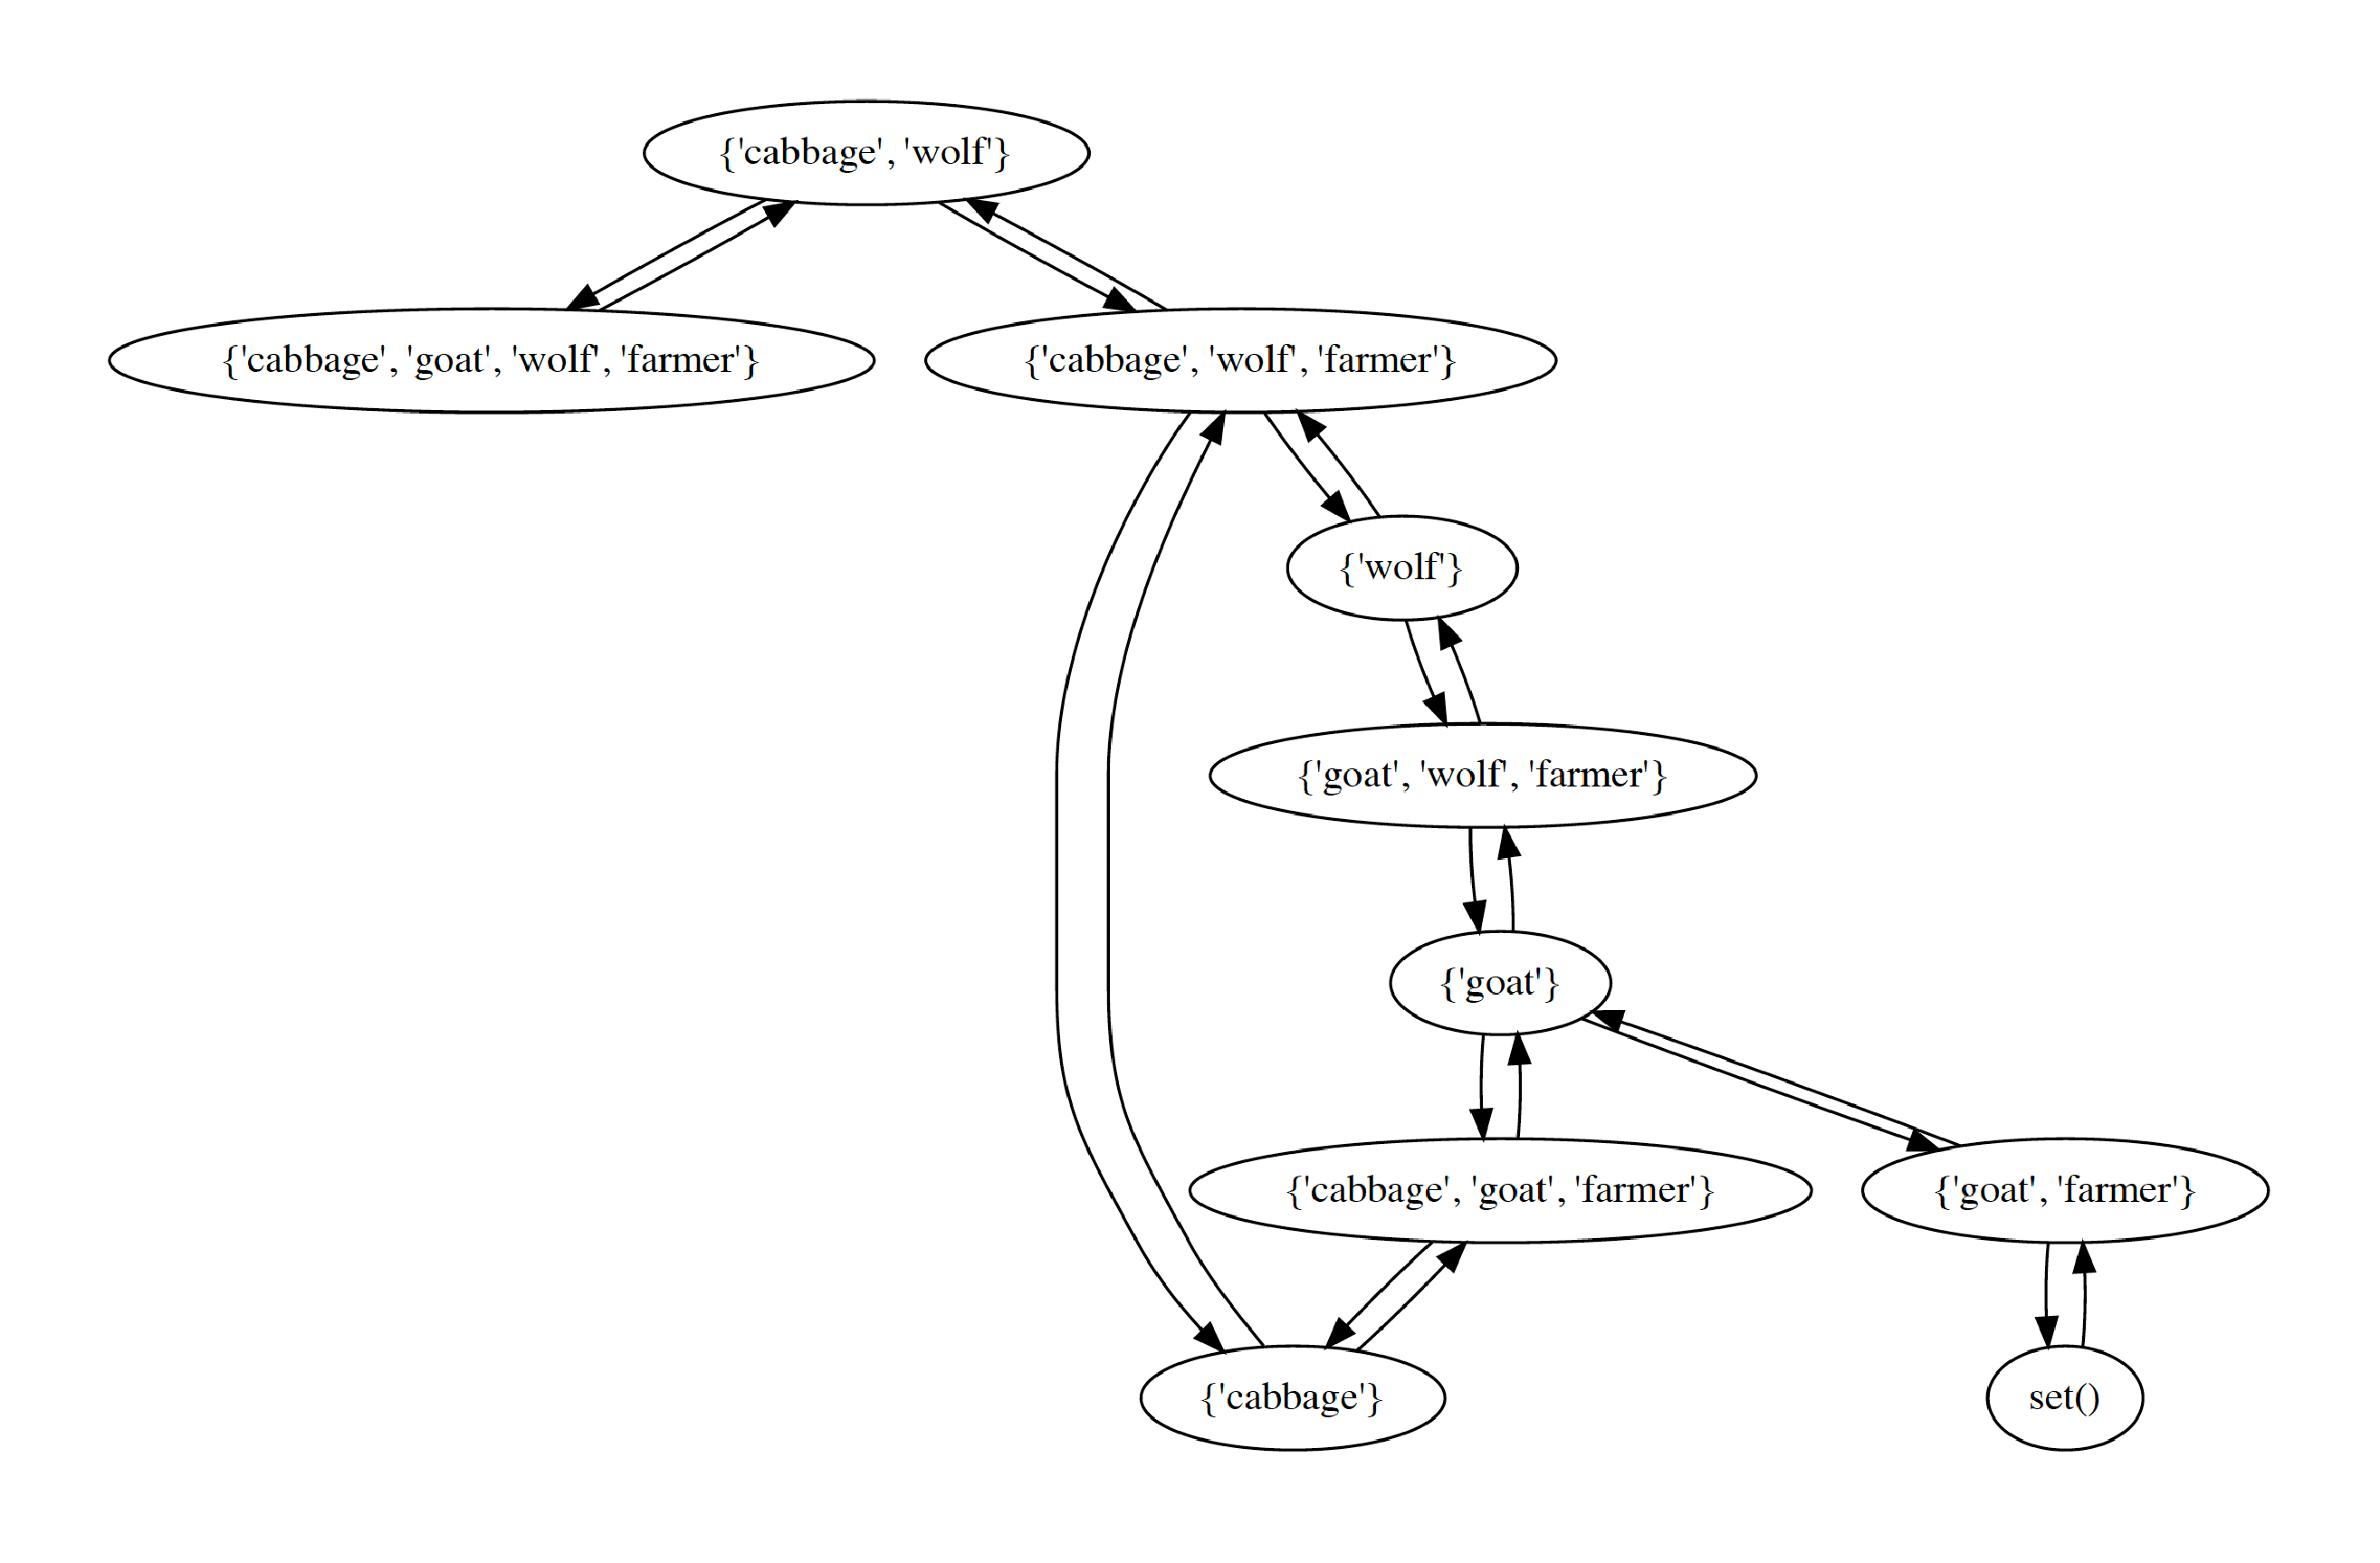
\epsfig{file=Figures/wolf-goat-cabbage, scale=0.4}

  \caption{The relation \texttt{R} shown as a directed graph.}
  \label{fig:wolf-goat-cabbage.pdf}
\end{figure}



\noindent
Figure \ref{fig:wolf-goat-cabbage.pdf} on page \pageref{fig:wolf-goat-cabbage.pdf} displays the relation $R$ graphically.
Figure \ref{fig:wolf-ziege} on page \pageref{fig:wolf-ziege} shows the program
\href{https://github.com/karlstroetmann/Logic/blob/master/Python/wolf-goat-cabbage.py}{\texttt{wolf-goat-cabbage.py}}
that combines the statements shown so far.  The solution computed by this program is shown in Figure
 \ref{fig:wolf-ziege-solution}.

\begin{figure}[!ht]
  \centering
\begin{minted}[ frame         = lines, 
                framesep      = 0.3cm, 
                numbers       = left,
                numbersep     = -0.2cm,
                bgcolor       = bg,
                xleftmargin   = 0.3cm,
                xrightmargin  = 0.3cm,
              ]{python3}
    def problem(S):
        return ('farmer' not in S) and             \
               (('goat' in S and 'cabbage' in S) or   # goat eats cabbage
                ('wolf' in S and 'goat'    in S)   )  # wolf eats goat
    
    All   = frozenset({ 'farmer', 'wolf', 'goat', 'cabbage' })
    R1    = { (S, S - B) for S in States for B in power(S)
                         if S - B in States and 'farmer' in B and len(B) <= 2
            }
    R2    = { (S2, S1) for (S1, S2) in R1 }
    R     = R1 | R2
    start = All
    goal  = frozenset()
    Path  = findPath(start, goal, R)
\end{minted} 
\vspace*{-0.3cm}
\caption{Solving the wolf-goat-cabbage problem.}  
\label{fig:wolf-ziege}
\end{figure}


\begin{figure}[!ht]
  \centering
\begin{minted}[ frame         = lines, 
                framesep      = 0.3cm, 
                numbers       = left,
                numbersep     = -0.2cm,
                bgcolor       = bg,
                xleftmargin   = 0.8cm,
                xrightmargin  = 0.8cm,
              ]{python3}
    {'cabbage', 'farmer', 'goat', 'wolf'}                                 {}
                             >>>> {'farmer', 'goat'} >>>> 
    {'cabbage', 'wolf'}                                   {'farmer', 'goat'}
                             <<<< {'farmer'} <<<< 
    {'cabbage', 'farmer', 'wolf'}                                   {'goat'}
                             >>>> {'farmer', 'wolf'} >>>> 
    {'cabbage'}                                   {'farmer', 'goat', 'wolf'}
                             <<<< {'farmer', 'goat'} <<<< 
    {'cabbage', 'farmer', 'goat'}                                   {'wolf'}
                             >>>> {'cabbage', 'farmer'} >>>> 
    {'goat'}                                   {'cabbage', 'farmer', 'wolf'}
                             <<<< {'farmer'} <<<< 
    {'farmer', 'goat'}                                   {'cabbage', 'wolf'}
                             >>>> {'farmer', 'goat'} >>>> 
    {}                                 {'cabbage', 'farmer', 'goat', 'wolf'}
\end{minted} 
\vspace*{-0.3cm}
\caption{A schedule for the agricultural economist.}  
\label{fig:wolf-ziege-solution}
\end{figure}

\vspace*{\fill}

%%% Local Variables:
%%% mode: latex
%%% TeX-master: "haskell"
%%% End:


\bibliographystyle{alpha}
\bibliography{cs}



\end{document}




%%% Local Variables:
%%% mode: latex
%%% TeX-master: t
g%%% End:
